% ==========================================================================
% INFO 4617 Web Data Science -- Week 6: Parsing Static Web Pages (Chapter 6)
% Build:  latexmk -pdf week-06.tex   (from this folder; no env vars needed)
% (or run `make` from the slides/ directory to build every deck)
% ==========================================================================
\documentclass[9pt,aspectratio=169]{beamer}
% Resolve the shared theme/preamble in ../common/ when compiling this
% file directly from its own folder (no TEXINPUTS needed).
\makeatletter\def\input@path{{../common/}}\makeatother
% ==========================================================================
% Shared preamble for INFO 4617 Web Data Science weekly lecture decks
% Based on the Gotham beamer theme (vendored in this directory).
% Each week's slides.tex does:  % ==========================================================================
% Shared preamble for INFO 4617 Web Data Science weekly lecture decks
% Based on the Gotham beamer theme (vendored in this directory).
% Each week's slides.tex does:  % ==========================================================================
% Shared preamble for INFO 4617 Web Data Science weekly lecture decks
% Based on the Gotham beamer theme (vendored in this directory).
% Each week's slides.tex does:  \input{preamble}  (with common/ on TEXINPUTS)
% then sets \title/\subtitle/\author/\date and \begin{document}.
% ==========================================================================

\usetheme{gotham}

\usepackage{fbb}
\usepackage{booktabs}
\usepackage{graphicx}
\usepackage{tikz}
\usepackage{xcolor}
\usepackage{multirow}
\usepackage{listings}
\usetikzlibrary{positioning, arrows.meta, shapes}

% Bibliography
\usepackage[style=authoryear,
            backend=biber,
            maxcitenames=1,
            uniquename=false,
            uniquelist=false]{biblatex}
\addbibresource{bibliography.bib}

\gothamset{sectiontocframe default=off}

% ------------------------------------------------------------------ colors
\definecolor{cugold}{HTML}{CFB87C}
\definecolor{tab-red}{HTML}{E15759}
\definecolor{tab-orange}{HTML}{F28E2B}
\definecolor{tab-blue}{HTML}{4E79A7}
\definecolor{tab-cyan}{HTML}{76B7B2}
\definecolor{tab-green}{HTML}{59A14F}
\definecolor{tab-yellow}{HTML}{EDC948}
\definecolor{tab-purple}{HTML}{B07AA1}
\definecolor{tab-pink}{HTML}{FF9DA7}
\definecolor{tab-brown}{HTML}{9C755F}
\definecolor{tab-gray}{HTML}{BAB0AC}

\setbeamercolor{frametitle}{fg=black, bg=cugold}
\setbeamercolor{progress bar}{fg=cugold, bg=cugold!20}

\setbeamercolor{block title alerted}{fg=black, bg=cugold}
\setbeamercolor{block body alerted}{fg=black, bg=cugold!10}

% ------------------------------------------------------------------ footline
\setbeamertemplate{footline}{
  \begin{beamercolorbox}[wd=\paperwidth,ht=2.5ex,dp=1ex,right]{footline}
    {\footnotesize \insertframenumber{} of \inserttotalframenumber}
    \hspace*{2ex}
  \end{beamercolorbox}
}

% ------------------------------------------------------------------ helpers
\newcommand{\bottomcite}[1]{
    \vspace*{\fill}
    \vspace{-\baselineskip}
    {\tiny
    \rule{\textwidth}{0.3pt}\\
    #1
    }
    \vspace{0.5ex}
}

% Consistent code styling for the Wednesday "applied notebook" frames.
\lstdefinestyle{wds}{
    basicstyle=\ttfamily\scriptsize,
    keywordstyle=\color{tab-blue}\bfseries,
    commentstyle=\color{tab-green},
    stringstyle=\color{tab-orange},
    showstringspaces=false,
    breaklines=true,
    columns=fullflexible,
    language=Python,
    aboveskip=0.4em,
    belowskip=0.4em,
}
\lstset{style=wds}

% \dayband{Day}{Topic} -- a lightweight section divider label used to mark
% Monday / Wednesday / Friday within a week's deck.
\newcommand{\dayband}[2]{{\large\textbf{#1}}\;\textcolor{tab-gray}{\textbar}\;#2}
  (with common/ on TEXINPUTS)
% then sets \title/\subtitle/\author/\date and \begin{document}.
% ==========================================================================

\usetheme{gotham}

\usepackage{fbb}
\usepackage{booktabs}
\usepackage{graphicx}
\usepackage{tikz}
\usepackage{xcolor}
\usepackage{multirow}
\usepackage{listings}
\usetikzlibrary{positioning, arrows.meta, shapes}

% Bibliography
\usepackage[style=authoryear,
            backend=biber,
            maxcitenames=1,
            uniquename=false,
            uniquelist=false]{biblatex}
\addbibresource{bibliography.bib}

\gothamset{sectiontocframe default=off}

% ------------------------------------------------------------------ colors
\definecolor{cugold}{HTML}{CFB87C}
\definecolor{tab-red}{HTML}{E15759}
\definecolor{tab-orange}{HTML}{F28E2B}
\definecolor{tab-blue}{HTML}{4E79A7}
\definecolor{tab-cyan}{HTML}{76B7B2}
\definecolor{tab-green}{HTML}{59A14F}
\definecolor{tab-yellow}{HTML}{EDC948}
\definecolor{tab-purple}{HTML}{B07AA1}
\definecolor{tab-pink}{HTML}{FF9DA7}
\definecolor{tab-brown}{HTML}{9C755F}
\definecolor{tab-gray}{HTML}{BAB0AC}

\setbeamercolor{frametitle}{fg=black, bg=cugold}
\setbeamercolor{progress bar}{fg=cugold, bg=cugold!20}

\setbeamercolor{block title alerted}{fg=black, bg=cugold}
\setbeamercolor{block body alerted}{fg=black, bg=cugold!10}

% ------------------------------------------------------------------ footline
\setbeamertemplate{footline}{
  \begin{beamercolorbox}[wd=\paperwidth,ht=2.5ex,dp=1ex,right]{footline}
    {\footnotesize \insertframenumber{} of \inserttotalframenumber}
    \hspace*{2ex}
  \end{beamercolorbox}
}

% ------------------------------------------------------------------ helpers
\newcommand{\bottomcite}[1]{
    \vspace*{\fill}
    \vspace{-\baselineskip}
    {\tiny
    \rule{\textwidth}{0.3pt}\\
    #1
    }
    \vspace{0.5ex}
}

% Consistent code styling for the Wednesday "applied notebook" frames.
\lstdefinestyle{wds}{
    basicstyle=\ttfamily\scriptsize,
    keywordstyle=\color{tab-blue}\bfseries,
    commentstyle=\color{tab-green},
    stringstyle=\color{tab-orange},
    showstringspaces=false,
    breaklines=true,
    columns=fullflexible,
    language=Python,
    aboveskip=0.4em,
    belowskip=0.4em,
}
\lstset{style=wds}

% \dayband{Day}{Topic} -- a lightweight section divider label used to mark
% Monday / Wednesday / Friday within a week's deck.
\newcommand{\dayband}[2]{{\large\textbf{#1}}\;\textcolor{tab-gray}{\textbar}\;#2}
  (with common/ on TEXINPUTS)
% then sets \title/\subtitle/\author/\date and \begin{document}.
% ==========================================================================

\usetheme{gotham}

\usepackage{fbb}
\usepackage{booktabs}
\usepackage{graphicx}
\usepackage{tikz}
\usepackage{xcolor}
\usepackage{multirow}
\usepackage{listings}
\usetikzlibrary{positioning, arrows.meta, shapes}

% Bibliography
\usepackage[style=authoryear,
            backend=biber,
            maxcitenames=1,
            uniquename=false,
            uniquelist=false]{biblatex}
\addbibresource{bibliography.bib}

\gothamset{sectiontocframe default=off}

% ------------------------------------------------------------------ colors
\definecolor{cugold}{HTML}{CFB87C}
\definecolor{tab-red}{HTML}{E15759}
\definecolor{tab-orange}{HTML}{F28E2B}
\definecolor{tab-blue}{HTML}{4E79A7}
\definecolor{tab-cyan}{HTML}{76B7B2}
\definecolor{tab-green}{HTML}{59A14F}
\definecolor{tab-yellow}{HTML}{EDC948}
\definecolor{tab-purple}{HTML}{B07AA1}
\definecolor{tab-pink}{HTML}{FF9DA7}
\definecolor{tab-brown}{HTML}{9C755F}
\definecolor{tab-gray}{HTML}{BAB0AC}

\setbeamercolor{frametitle}{fg=black, bg=cugold}
\setbeamercolor{progress bar}{fg=cugold, bg=cugold!20}

\setbeamercolor{block title alerted}{fg=black, bg=cugold}
\setbeamercolor{block body alerted}{fg=black, bg=cugold!10}

% ------------------------------------------------------------------ footline
\setbeamertemplate{footline}{
  \begin{beamercolorbox}[wd=\paperwidth,ht=2.5ex,dp=1ex,right]{footline}
    {\footnotesize \insertframenumber{} of \inserttotalframenumber}
    \hspace*{2ex}
  \end{beamercolorbox}
}

% ------------------------------------------------------------------ helpers
\newcommand{\bottomcite}[1]{
    \vspace*{\fill}
    \vspace{-\baselineskip}
    {\tiny
    \rule{\textwidth}{0.3pt}\\
    #1
    }
    \vspace{0.5ex}
}

% Consistent code styling for the Wednesday "applied notebook" frames.
\lstdefinestyle{wds}{
    basicstyle=\ttfamily\scriptsize,
    keywordstyle=\color{tab-blue}\bfseries,
    commentstyle=\color{tab-green},
    stringstyle=\color{tab-orange},
    showstringspaces=false,
    breaklines=true,
    columns=fullflexible,
    language=Python,
    aboveskip=0.4em,
    belowskip=0.4em,
}
\lstset{style=wds}

% \dayband{Day}{Topic} -- a lightweight section divider label used to mark
% Monday / Wednesday / Friday within a week's deck.
\newcommand{\dayband}[2]{{\large\textbf{#1}}\;\textcolor{tab-gray}{\textbar}\;#2}


\title[Week 6 · Static Pages]{{\Huge Parsing Static Web Pages}}
\subtitle{Week 6 · Documents module · Textbook Chapter 6}
\author[Keegan]{\textbf{Brian C. Keegan, Ph.D.} \\ Associate Professor, Department of Information Science \\ University of Colorado Boulder}
\date{September 21, 23 \& 25, 2026}

\begin{document}

\maketitle

% -------------------------------------------------------------------------
\begin{frame}{This week at a glance}
    \begin{columns}[T]
        \begin{column}{0.6\textwidth}
            We turn HTML --- the language of web pages --- into data you can analyze. Movies carry the examples all week: box office charts, Wikipedia film pages, and the Oscars.

            \bigskip

            \dayband{Monday}{Concepts \& notebook intro}
            \begin{itemize}\small
                \item Eight common shapes static pages hide their data in, and where each one sits on a single-site/multi-site, consistent/inconsistent design spectrum
            \end{itemize}

            \medskip

            \dayband{Wednesday}{Notebook lab}
            \begin{itemize}\small
                \item Pilot each strategy in code: box office, Wikipedia, the Oscars, and Rotten Tomatoes
            \end{itemize}

            \medskip

            \dayband{Friday}{Textbook revisions}
            \begin{itemize}\small
                \item Propose \& peer-review pull requests improving Chapter 6
            \end{itemize}
        \end{column}
        \begin{column}{0.35\textwidth}
            \begin{block}{Companion notebook}
                \footnotesize \texttt{ch-06-static-pages.ipynb}
            \end{block}
            \begin{alertblock}{Bring a laptop}
                \footnotesize Wednesday is hands-on --- we debug live.
            \end{alertblock}
        \end{column}
    \end{columns}
\end{frame}

% =========================================================================
\section{Monday · Concepts}
% =========================================================================

\begin{frame}{From HTML to data}
    \begin{columns}[T]
        \begin{column}{0.6\textwidth}
            The goal of scraping: convert one structured format --- HTML --- into another suited to analysis (a pandas DataFrame, CSV, or JSON).

            \bigskip

            HTML and XML are \textbf{siblings} (both descend from SGML), so your \texttt{BeautifulSoup} skills transfer directly.

            \bigskip

            But browsers \textit{tolerate} malformed markup --- unclosed tags, missing quotes, bad nesting --- so real HTML is far messier than clean XML.

            \bigskip

            The core skill this week: \textbf{cutting through the noise} of navigation bars, ads, tracking scripts, and nested \texttt{<div>}s to reach the data.
        \end{column}
        \begin{column}{0.35\textwidth}
            \centering
            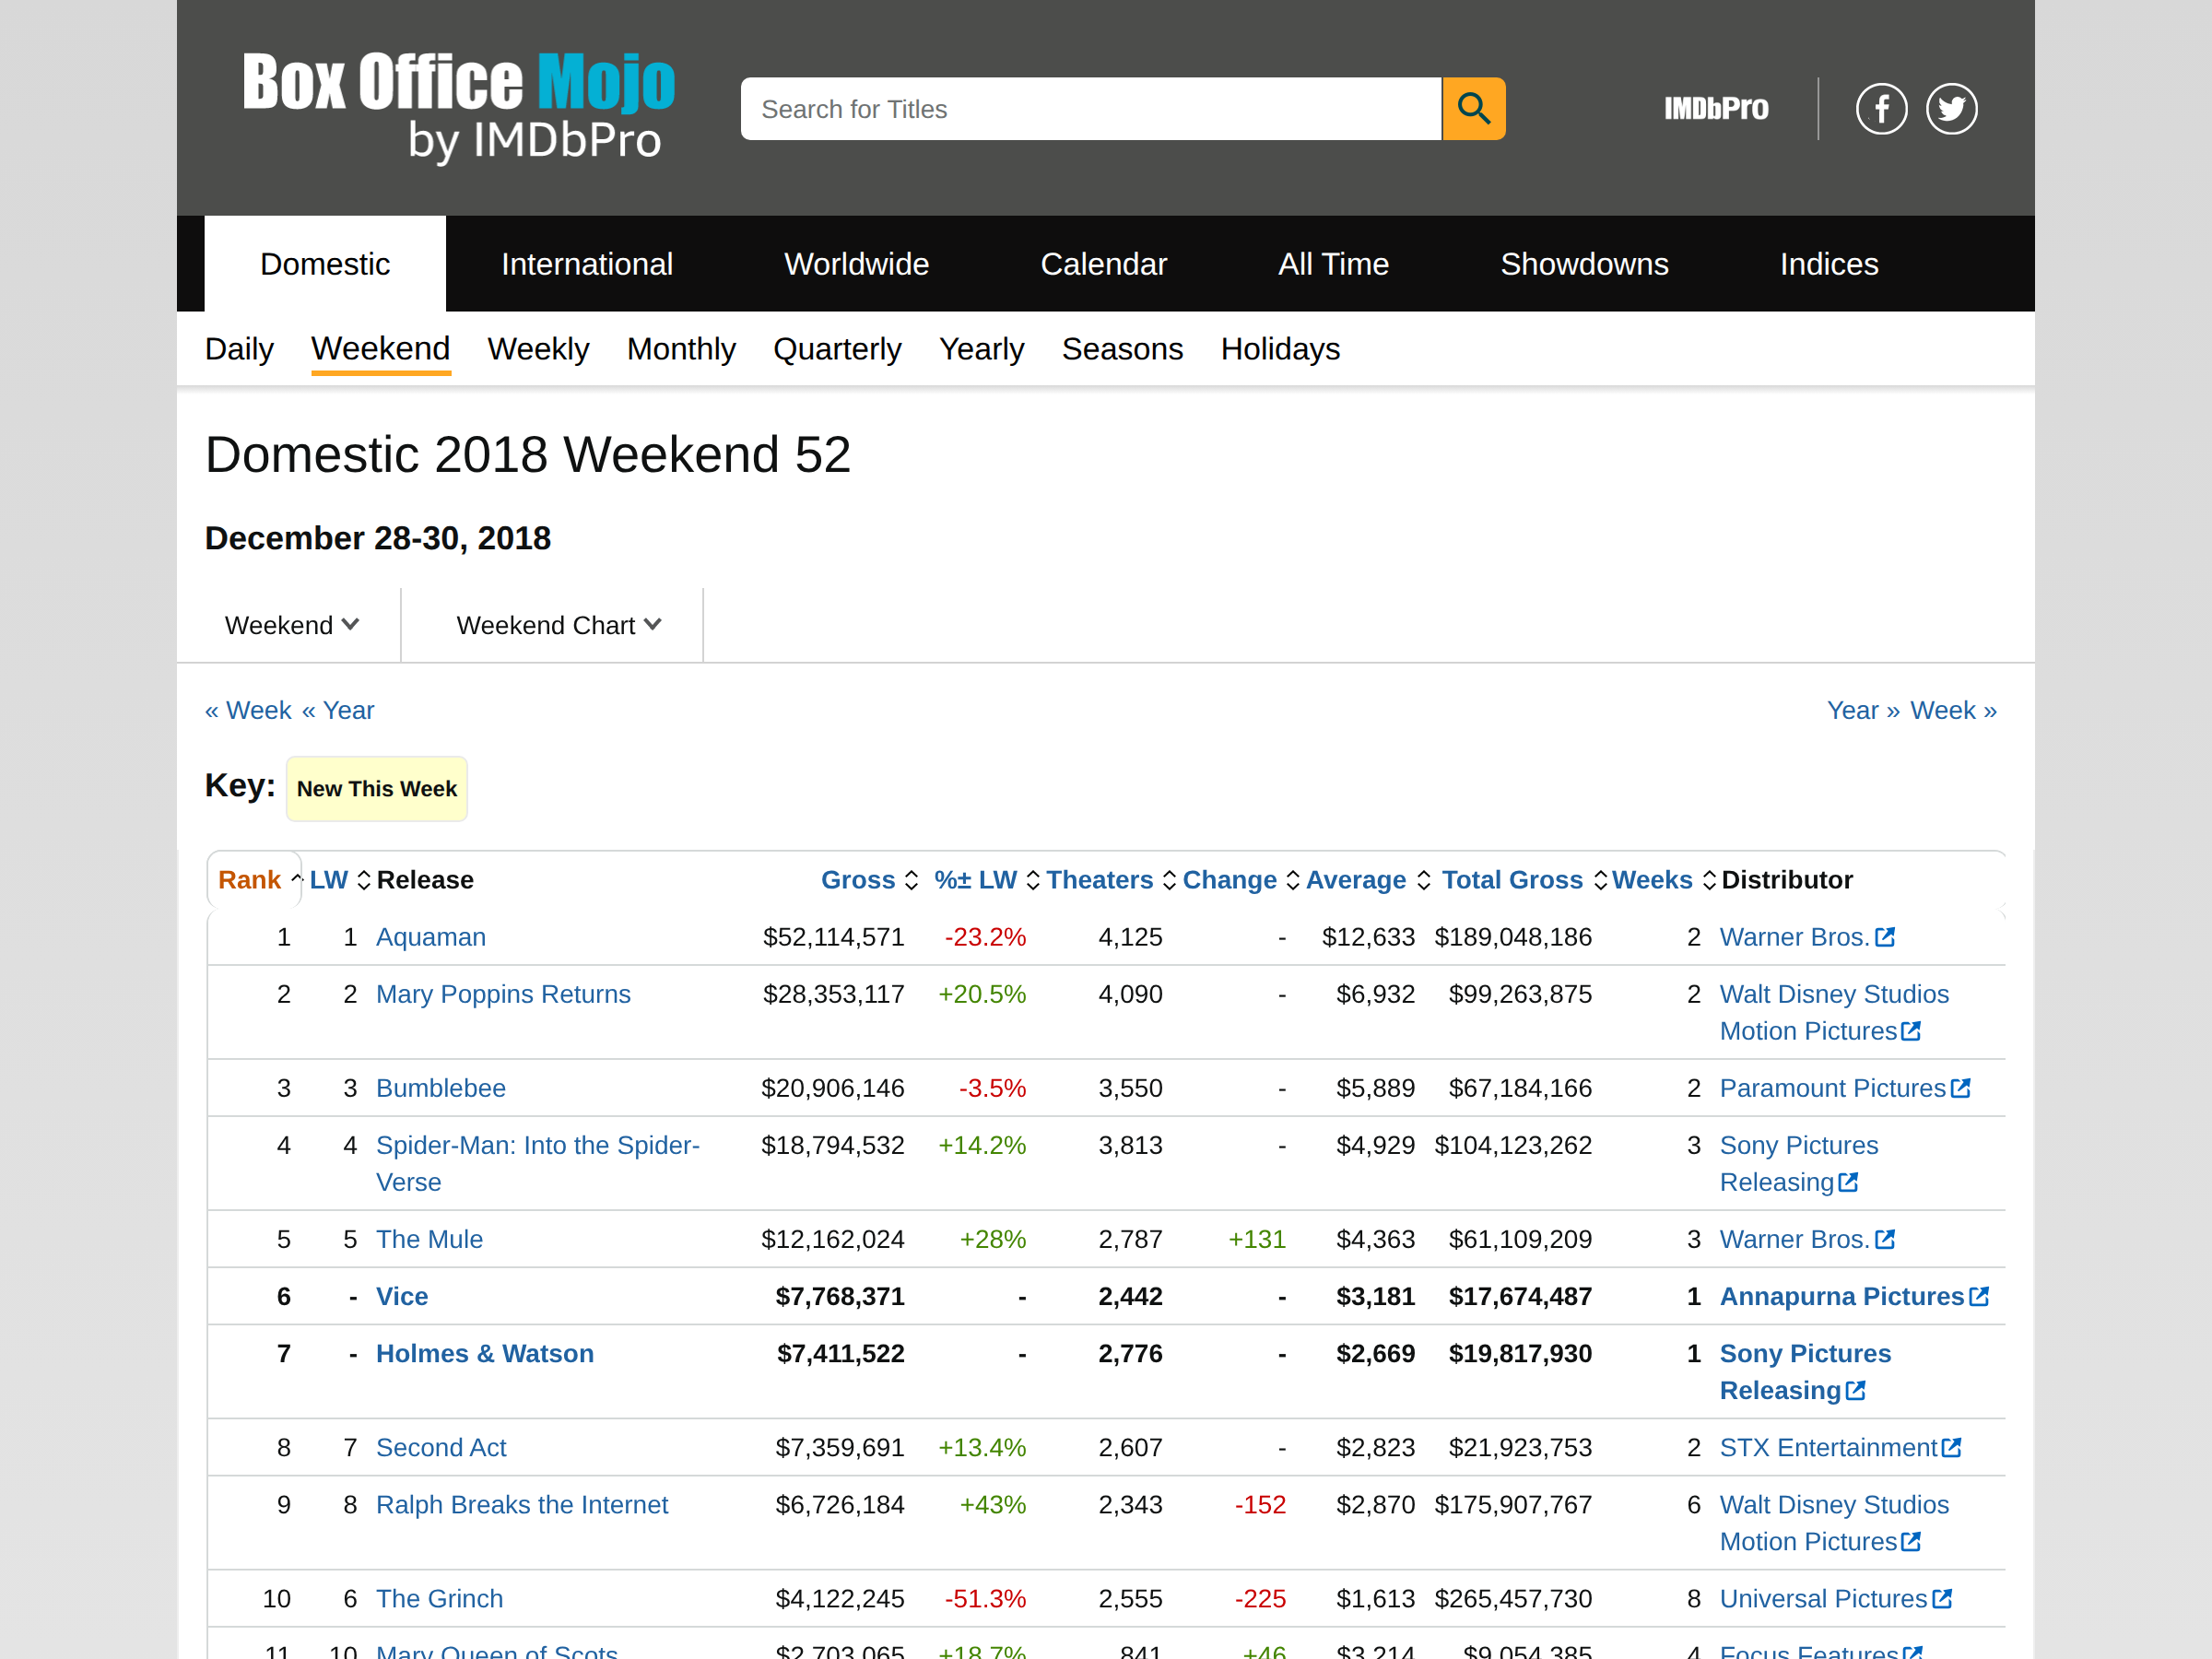
\includegraphics[width=\textwidth]{img/bom_weekly_chart.png}\\
            {\scriptsize A page with the data already sitting in one table.}
        \end{column}
    \end{columns}
\end{frame}

\begin{frame}{Inspect before you parse}
    \begin{columns}[T]
        \begin{column}{0.6\textwidth}
            Chapter 5 already put you in the Inspector: right-click the data, choose \textbf{Inspect}, and read the DOM the browser actually built.

            \bigskip

            Today that skill gets a narrower job. You are not exploring a page cold --- you already know your target is data. The only question is \textbf{which shape the data is hiding in}, and every shape below answers that question with a different look inside the Inspector.

            \bigskip

            One habit from Chapter 5 carries forward unchanged: if an element is visible in the Inspector but missing from \texttt{requests.get(url).text}, JavaScript put it there after the fact --- keep that in mind for Strategy 8.
        \end{column}
        \begin{column}{0.35\textwidth}
            \centering
            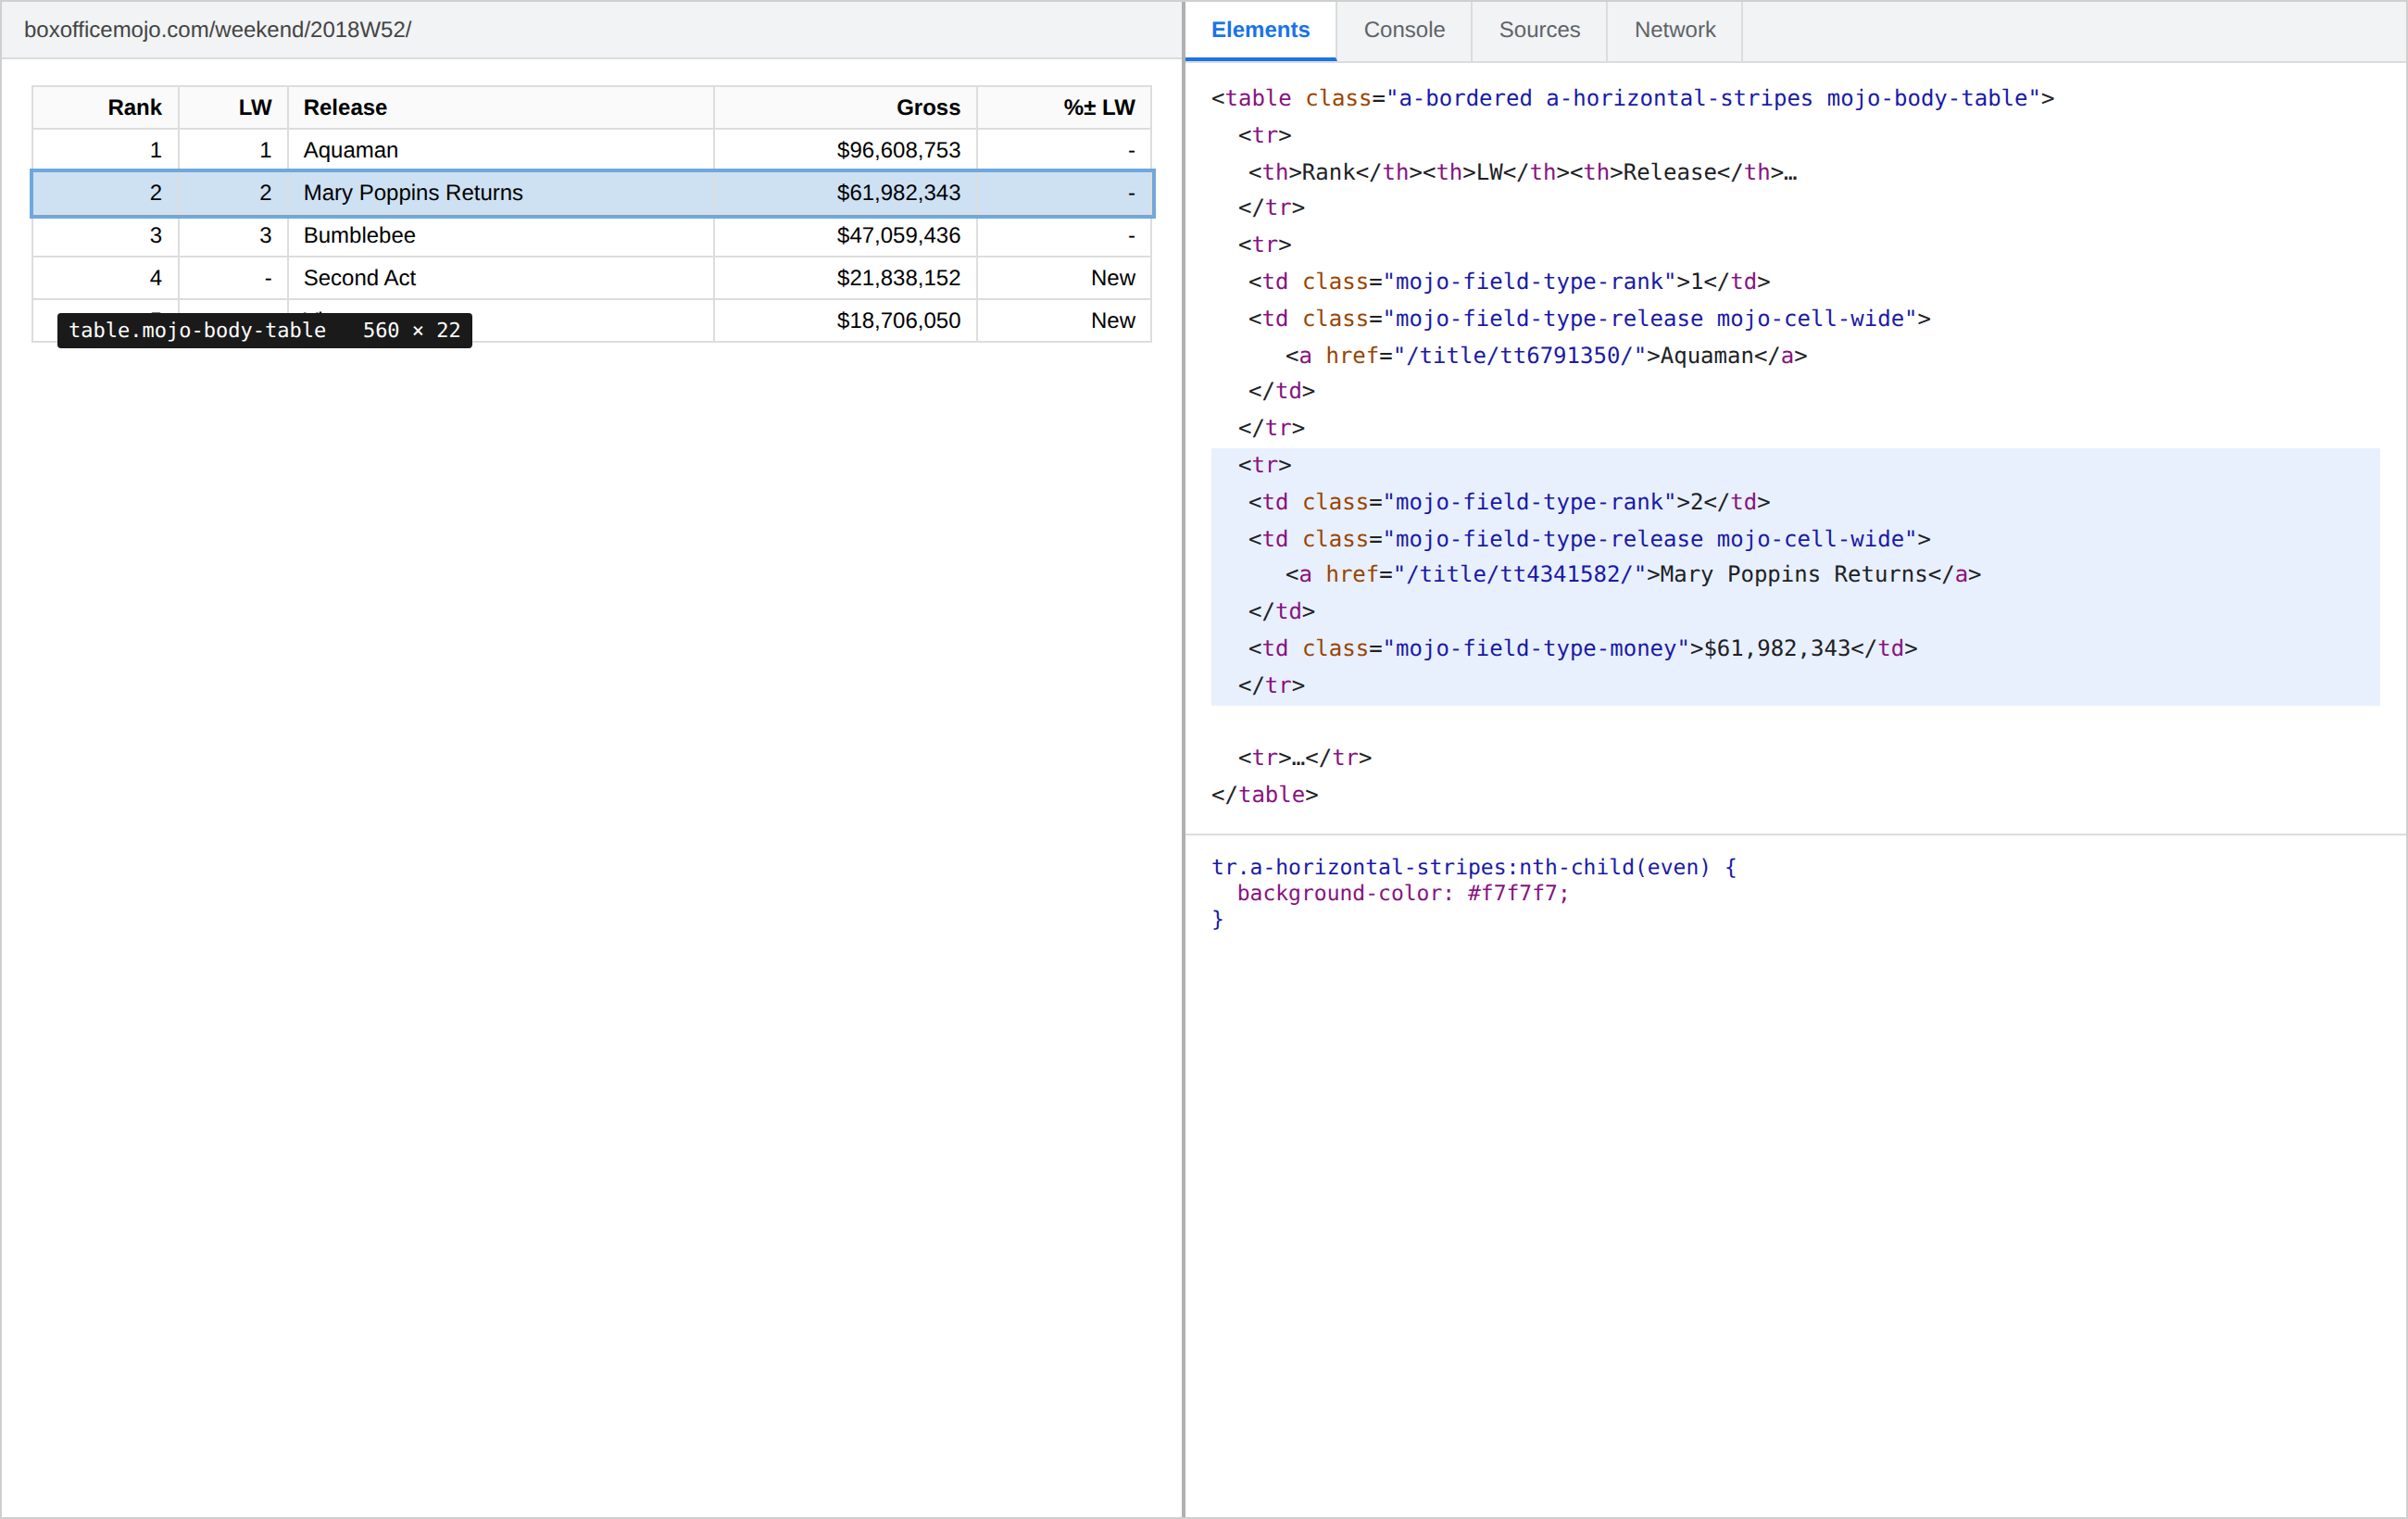
\includegraphics[width=\textwidth]{img/dev_tools_inspect.png}\\
            {\scriptsize The Elements panel on a real Box Office Mojo table.}
        \end{column}
    \end{columns}
\end{frame}

\begin{frame}{Common research designs: a 2$\times$2 spectrum}
    \begin{columns}[T]
        \begin{column}{0.55\textwidth}
            Before picking a parsing strategy, place your project on two axes: how many \textbf{sites} you're pulling from, and how \textbf{consistent} their design is page to page.
            \bigskip
            \begin{itemize}\small
                \item \textbf{Single site, consistent design.} Fifty-two weekly Box Office Mojo pages --- same template every time.
                \item \textbf{Single site, inconsistent design.} One oscars.org ceremony page where the winner's card and a nominee's card aren't shaped the same.
                \item \textbf{Multiple sites, consistent design.} English and French Wikipedia film infoboxes --- same platform, same idea, different specifics.
                \item \textbf{Multiple sites, inconsistent design.} The Numbers, Box Office Mojo, and Rotten Tomatoes --- three real sites, three unrelated HTML structures, for the same movies.
            \end{itemize}
        \end{column}
        \begin{column}{0.42\textwidth}
            \tiny
            \begin{tabular}{@{}p{1.1cm}p{2.0cm}p{2.0cm}@{}}
                 & \textbf{1 site} & \textbf{multi-site} \\ \hline
                \textbf{same design} & weekly BOM charts & EN/FR infoboxes \\[3pt] \hline
                \textbf{differs} & Oscars: winner vs.\ nominee & Numbers vs.\ Mojo vs.\ RT \\
            \end{tabular}
            \bigskip

            Complexity climbs left-to-right, top-to-bottom. Most real research projects live somewhere past the top-left cell.
        \end{column}
    \end{columns}
\end{frame}

\begin{frame}{Strategy 1 --- the clean single table}
    \begin{columns}[T]
        \begin{column}{0.6\textwidth}
            The best case: one table, one target, nothing else on the page competing for it.

            \bigskip

            Box Office Mojo's weekly chart is exactly this --- a single ranked table of that week's top movies. The moment you find it, you are basically done: no navigation tables, no decoys, no ambiguity about which element holds the data.

            \bigskip

            This is the case \texttt{pandas.read\_html()} was built for.
        \end{column}
        \begin{column}{0.35\textwidth}
            \centering
            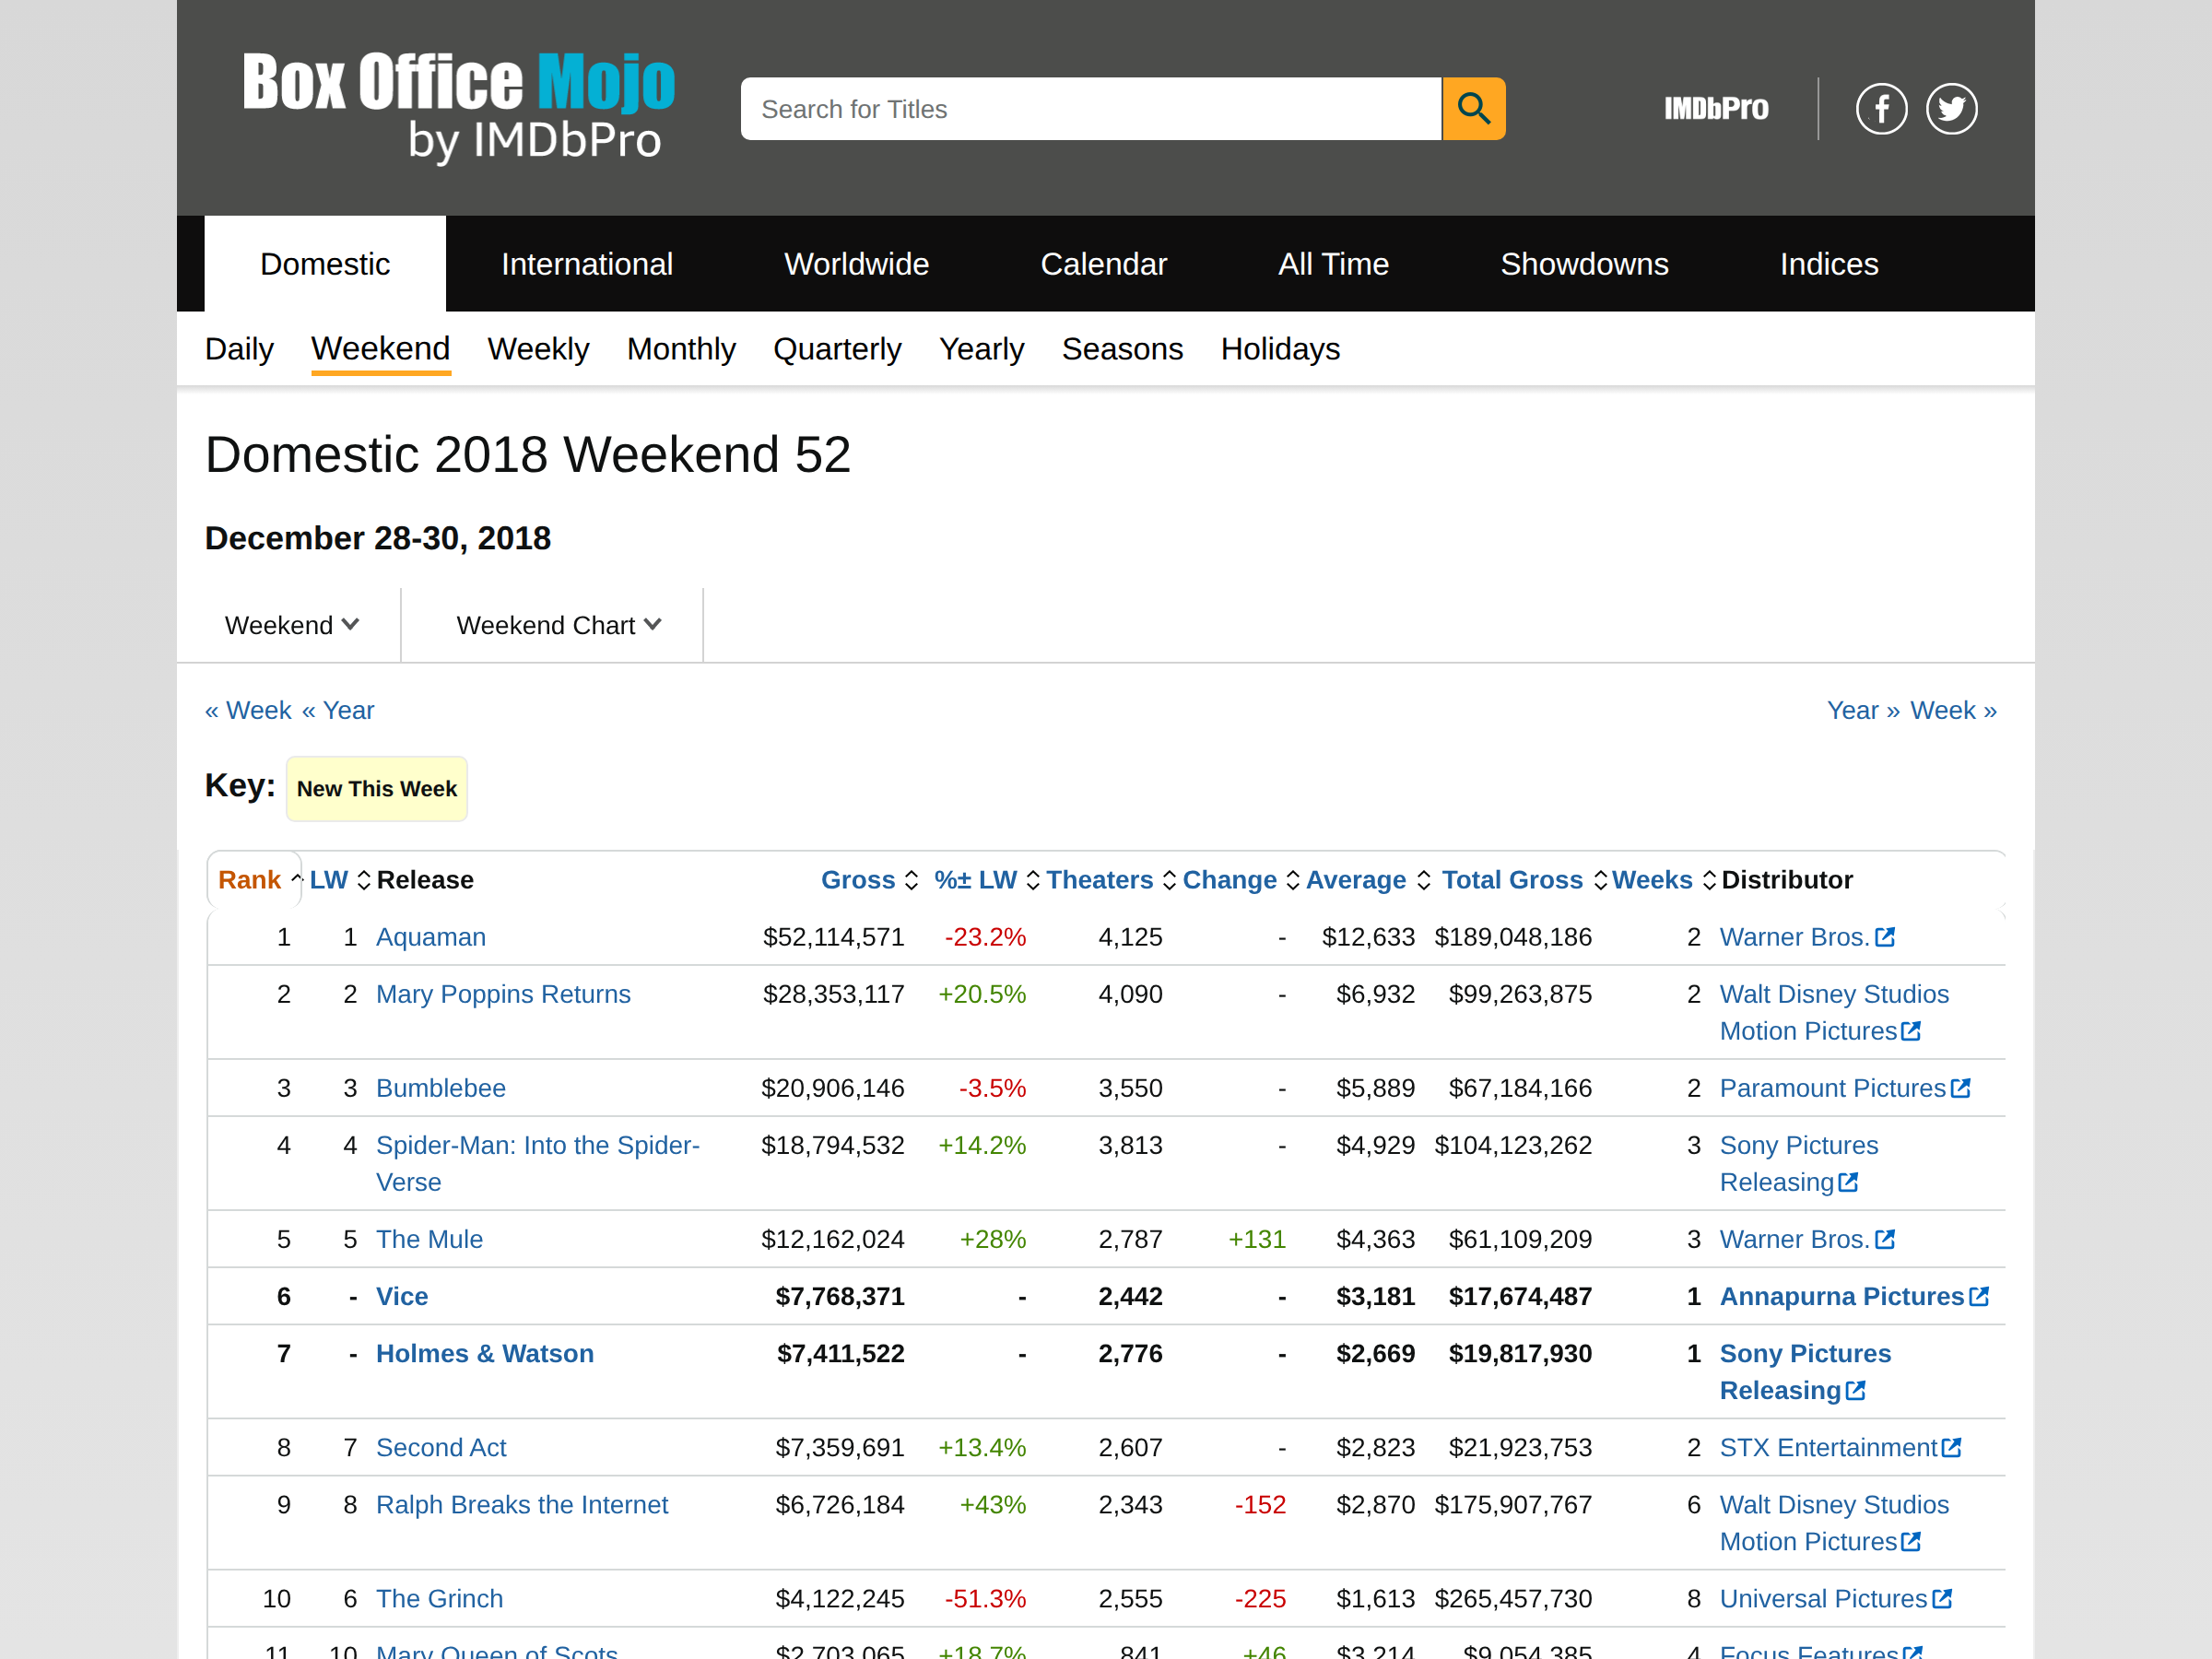
\includegraphics[width=\textwidth]{img/bom_weekly_chart.png}\\
            {\scriptsize boxofficemojo.com/weekend/2018W52/}
        \end{column}
    \end{columns}
\end{frame}

\begin{frame}{Strategy 2 --- a table hiding among decoys}
    \begin{columns}[T]
        \begin{column}{0.6\textwidth}
            Real pages are rarely this polite. The Numbers' weekly chart has the \textit{same kind} of data as Box Office Mojo, but its HTML ships \textbf{two} \texttt{<table>} elements --- a full desktop layout and a separate mobile layout --- and only one is the table you want.

            \bigskip

            Same site, same page, same intent as Strategy 1 --- but now you must inspect and count before you trust \texttt{find\_all("table")[0]}.
        \end{column}
        \begin{column}{0.35\textwidth}
            \centering
            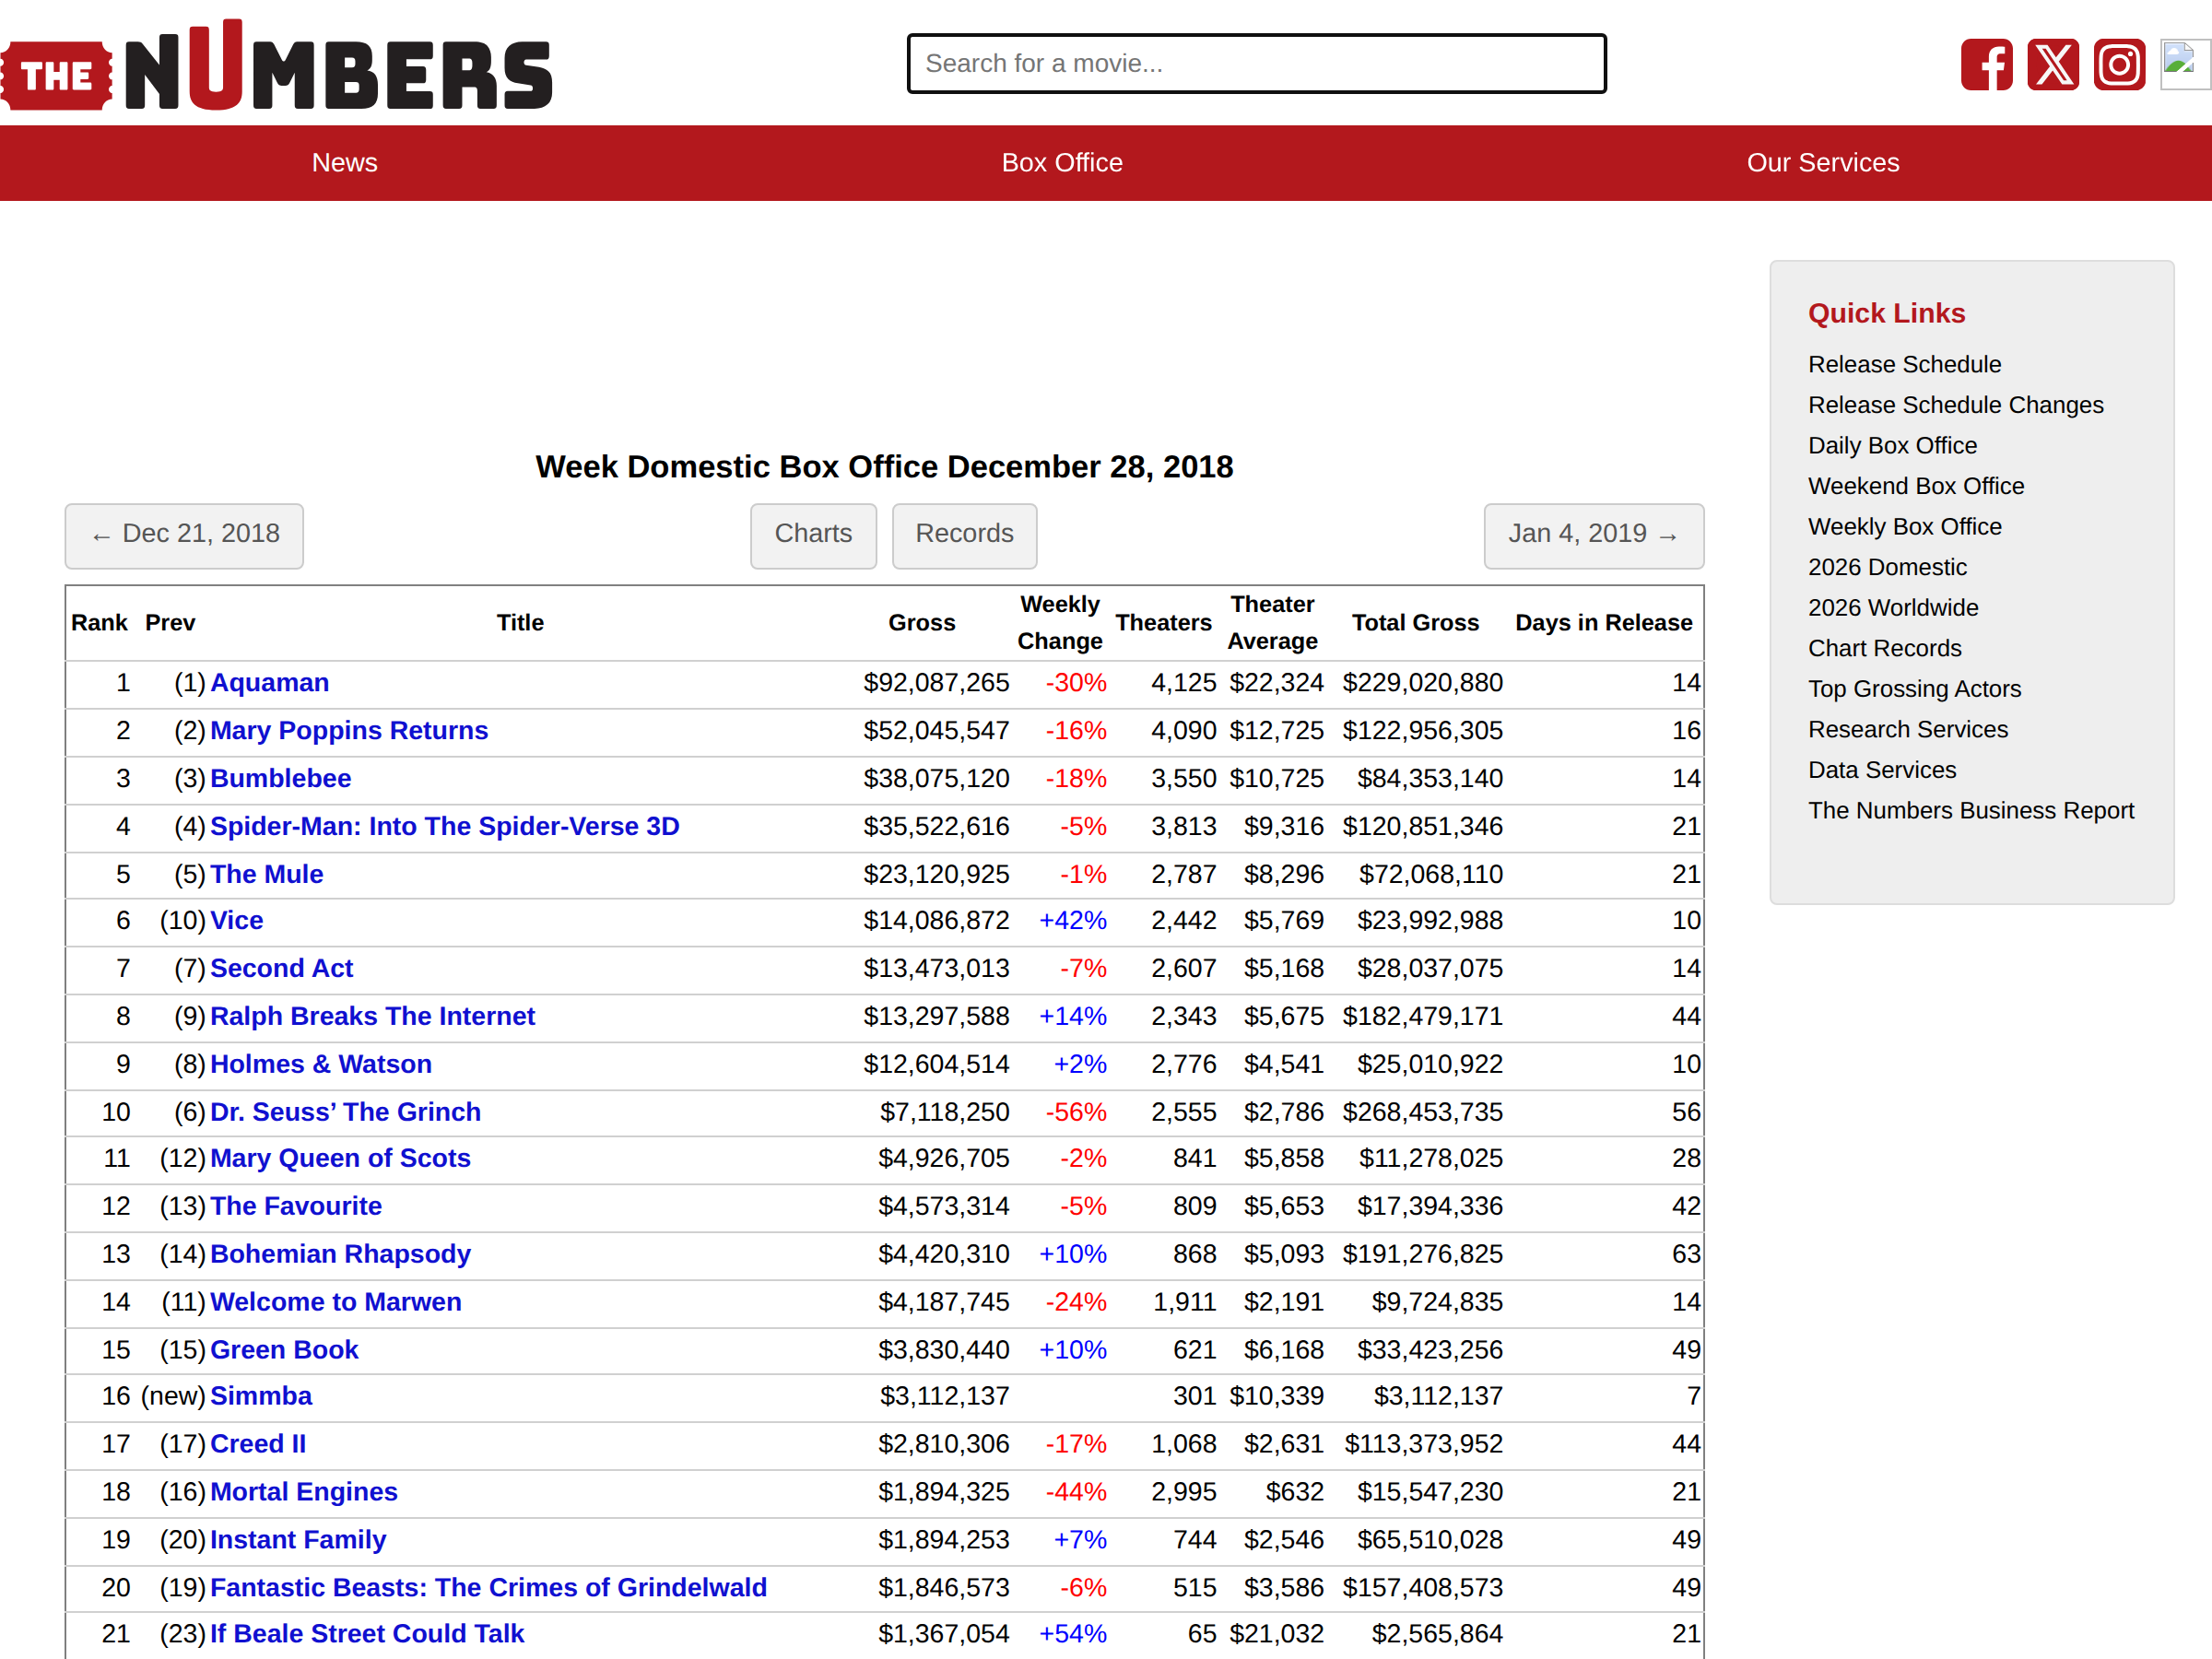
\includegraphics[width=\textwidth]{img/the_numbers_table.png}\\
            {\scriptsize the-numbers.com --- two tables, one is the data.}
        \end{column}
    \end{columns}
\end{frame}

\begin{frame}{Strategy 3 --- the table that needs cleanup}
    \begin{columns}[T]
        \begin{column}{0.6\textwidth}
            Sometimes the table extracts cleanly and the \textit{values} don't. Wikipedia's ``List of highest-grossing films'' is the classic case: \texttt{read\_html()} succeeds on the first try, and the real work starts after.

            \bigskip

            Footnote markers glue onto titles. A stray superscript letter sits in front of some dollar amounts. Numbers arrive as text. None of this breaks extraction --- it breaks \textit{analysis} until you clean it.
        \end{column}
        \begin{column}{0.35\textwidth}
            \centering
            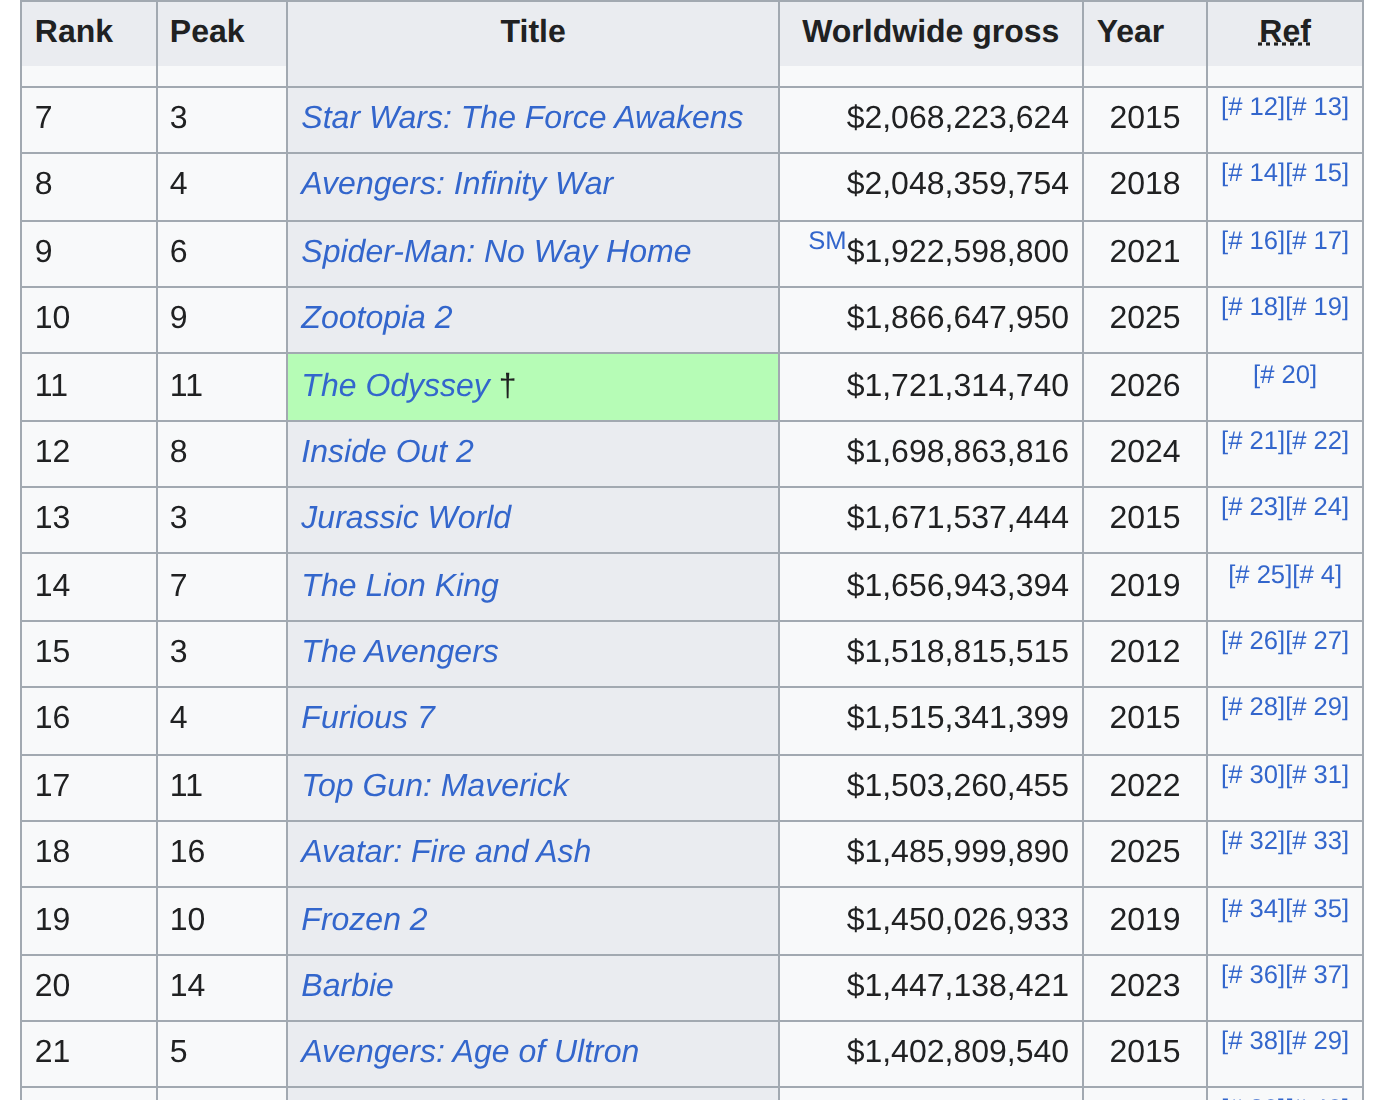
\includegraphics[width=\textwidth]{img/wiki_highest_grossing_table.png}\\
            {\scriptsize A table that parses fine and reads badly.}
        \end{column}
    \end{columns}
\end{frame}

\begin{frame}{Strategy 4 --- the infobox pattern}
    \begin{columns}[T]
        \begin{column}{0.6\textwidth}
            Not every page's real content lives inside a data \texttt{<table>}. Wikipedia's film infoboxes are a labeled key--value block --- ``Directed by,'' ``Produced by,'' ``Starring'' --- one row per fact, in roughly the same shape on every film's page.

            \bigskip

            Once you can pull one film's infobox apart, the same handful of lines pulls apart the next five hundred.
        \end{column}
        \begin{column}{0.35\textwidth}
            \centering
            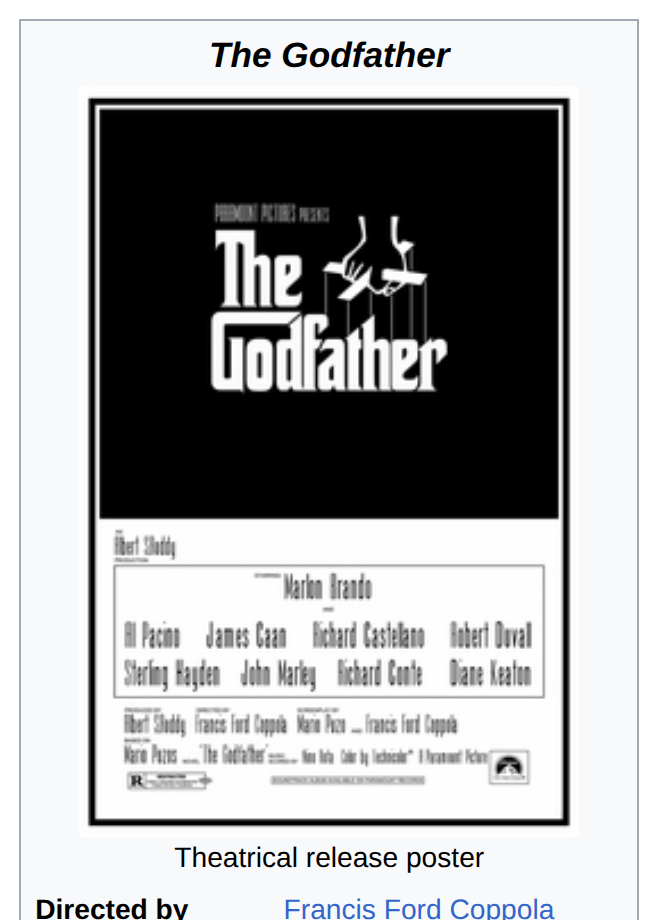
\includegraphics[width=\textwidth]{img/wiki_infobox_en.png}\\
            {\scriptsize en.wikipedia.org --- \textit{The Godfather}.}
        \end{column}
    \end{columns}
\end{frame}

\begin{frame}{Strategy 5 --- porting the pattern to a new site}
    \begin{columns}[T]
        \begin{column}{0.6\textwidth}
            The infobox idea from Strategy 4 isn't just reusable across English Wikipedia pages --- it travels to any site built on the same platform. French Wikipedia runs the same software and lays out its film infobox the same conceptual way.

            \bigskip

            But it is not the same page. The anchor that worked on the English article --- a table class name --- does not exist here at all; the reliable anchor turns out to be the table's \texttt{<caption>} instead. \textbf{The strategy transfers. The specific selector has to be re-verified, every time.}
        \end{column}
        \begin{column}{0.35\textwidth}
            \centering
            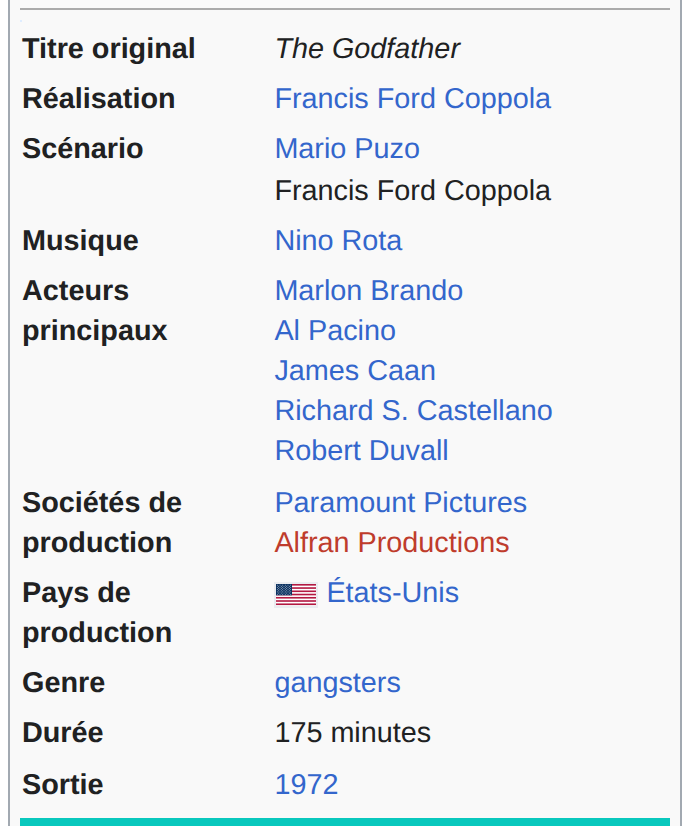
\includegraphics[width=\textwidth]{img/wiki_infobox_fr.png}\\
            {\scriptsize fr.wikipedia.org --- \textit{Le Parrain}, same idea.}
        \end{column}
    \end{columns}
\end{frame}

\begin{frame}{Strategy 6 --- cards that need to become rows}
    \begin{columns}[T]
        \begin{column}{0.6\textwidth}
            The Academy Awards' own site lists nominees and winners as a grid of individual cards --- one per category, holding several honorees --- with \textbf{no table anywhere on the page}.

            \bigskip

            Turning this into a DataFrame means treating each honoree as one row: find the repeating category container, then pull category name, winner-or-nominee status, person, and film out of each honoree inside it.

            \bigskip

            This is the shape behind most gallery and directory pages --- and the one static-page pattern that shows up the most once you start looking for it.
        \end{column}
        \begin{column}{0.35\textwidth}
            \centering
            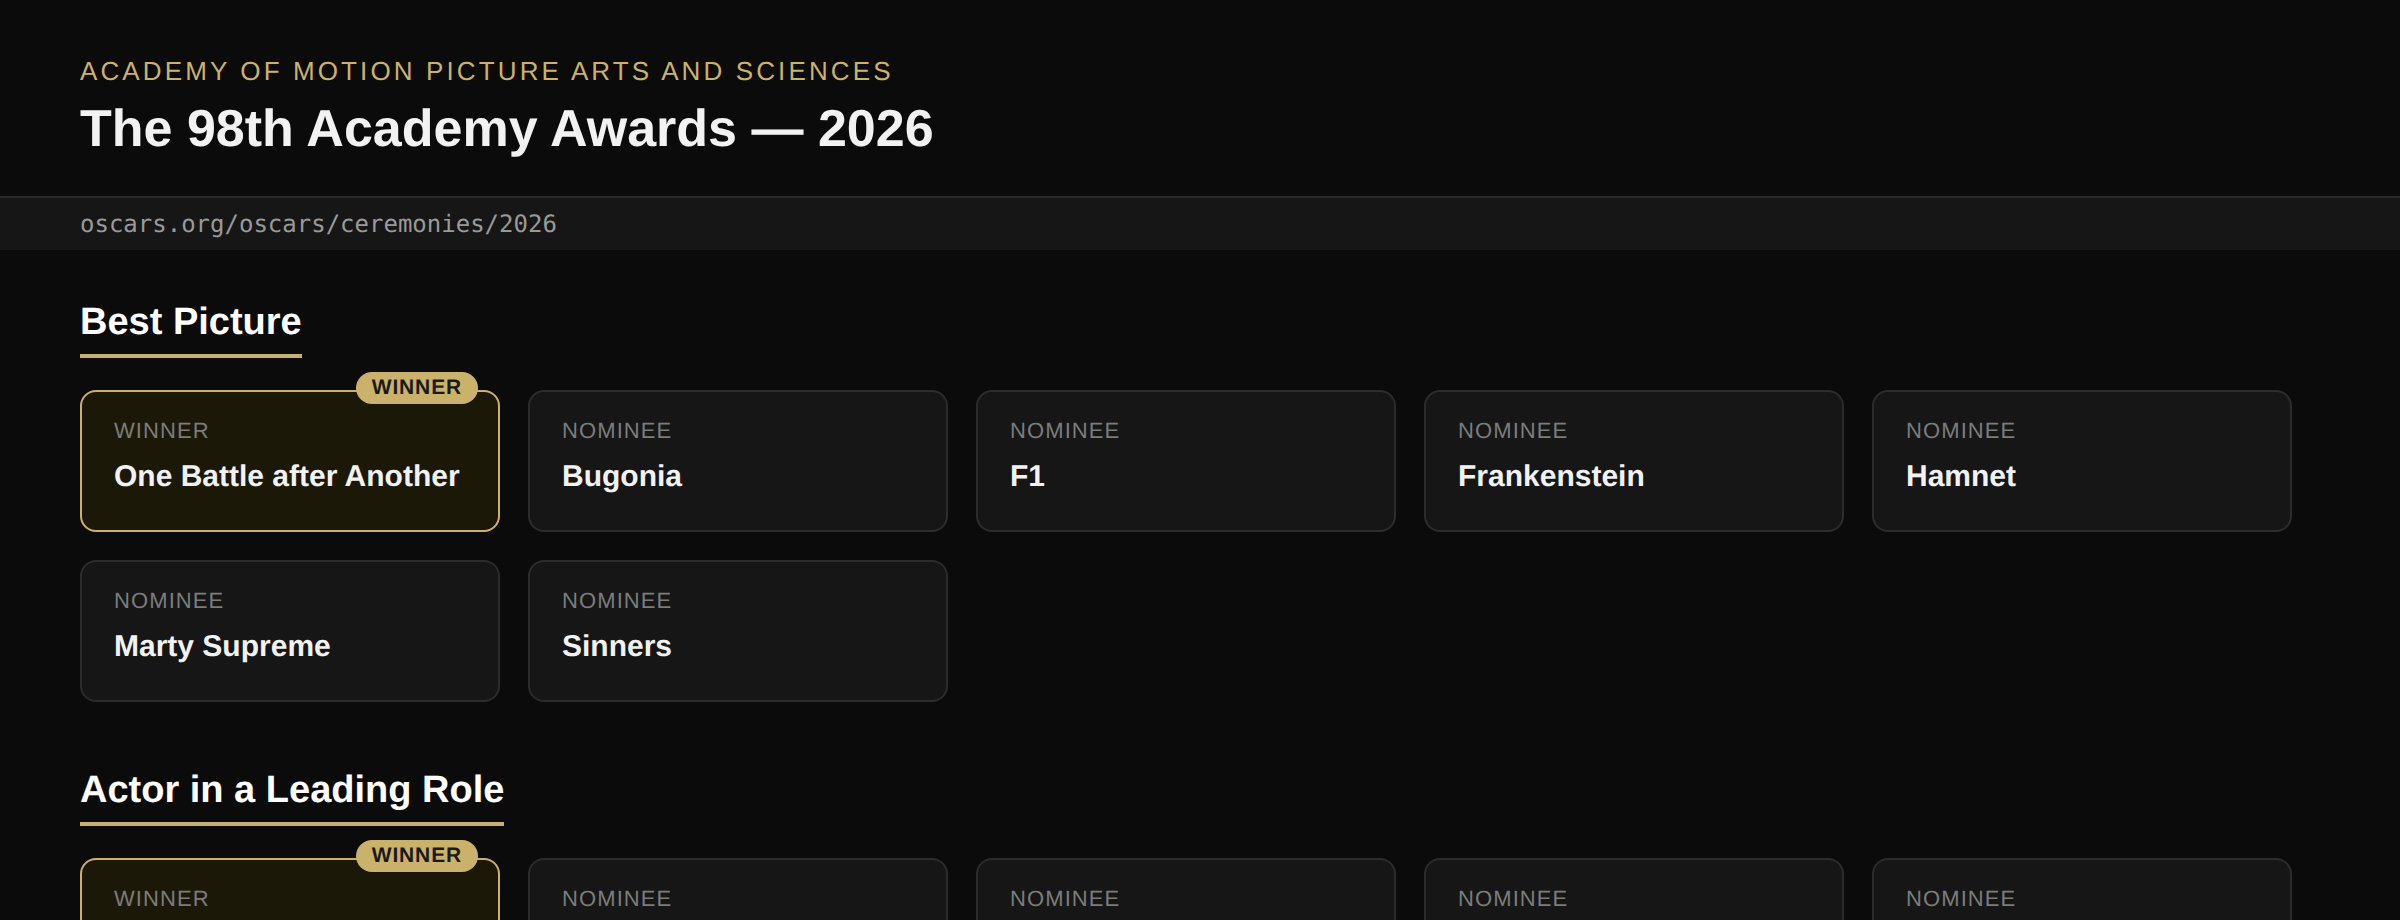
\includegraphics[width=\textwidth]{img/oscars_cards.png}\\
            {\scriptsize oscars.org --- 2026 ceremony, one card per honoree.}
        \end{column}
    \end{columns}
\end{frame}

\begin{frame}{Strategy 7 --- inconsistent cards, multiple sites}
    \begin{columns}[T]
        \begin{column}{0.6\textwidth}
            Rotten Tomatoes' ``Movies in Theaters'' grid looks like the same idea as the Oscars cards --- a repeating tile per movie --- but the tile itself is a different shape entirely: a poster, a title, and a Tomatometer score, built from custom elements instead of plain \texttt{<div>}s.

            \bigskip

            A research question that needs \textit{both} box-office numbers and critical reception can't use one parser for both sites. You write one card-parser per site, then reconcile the two into a single schema --- one row per movie --- afterward. This is the general shape of most real scraping pipelines.
        \end{column}
        \begin{column}{0.35\textwidth}
            \centering
            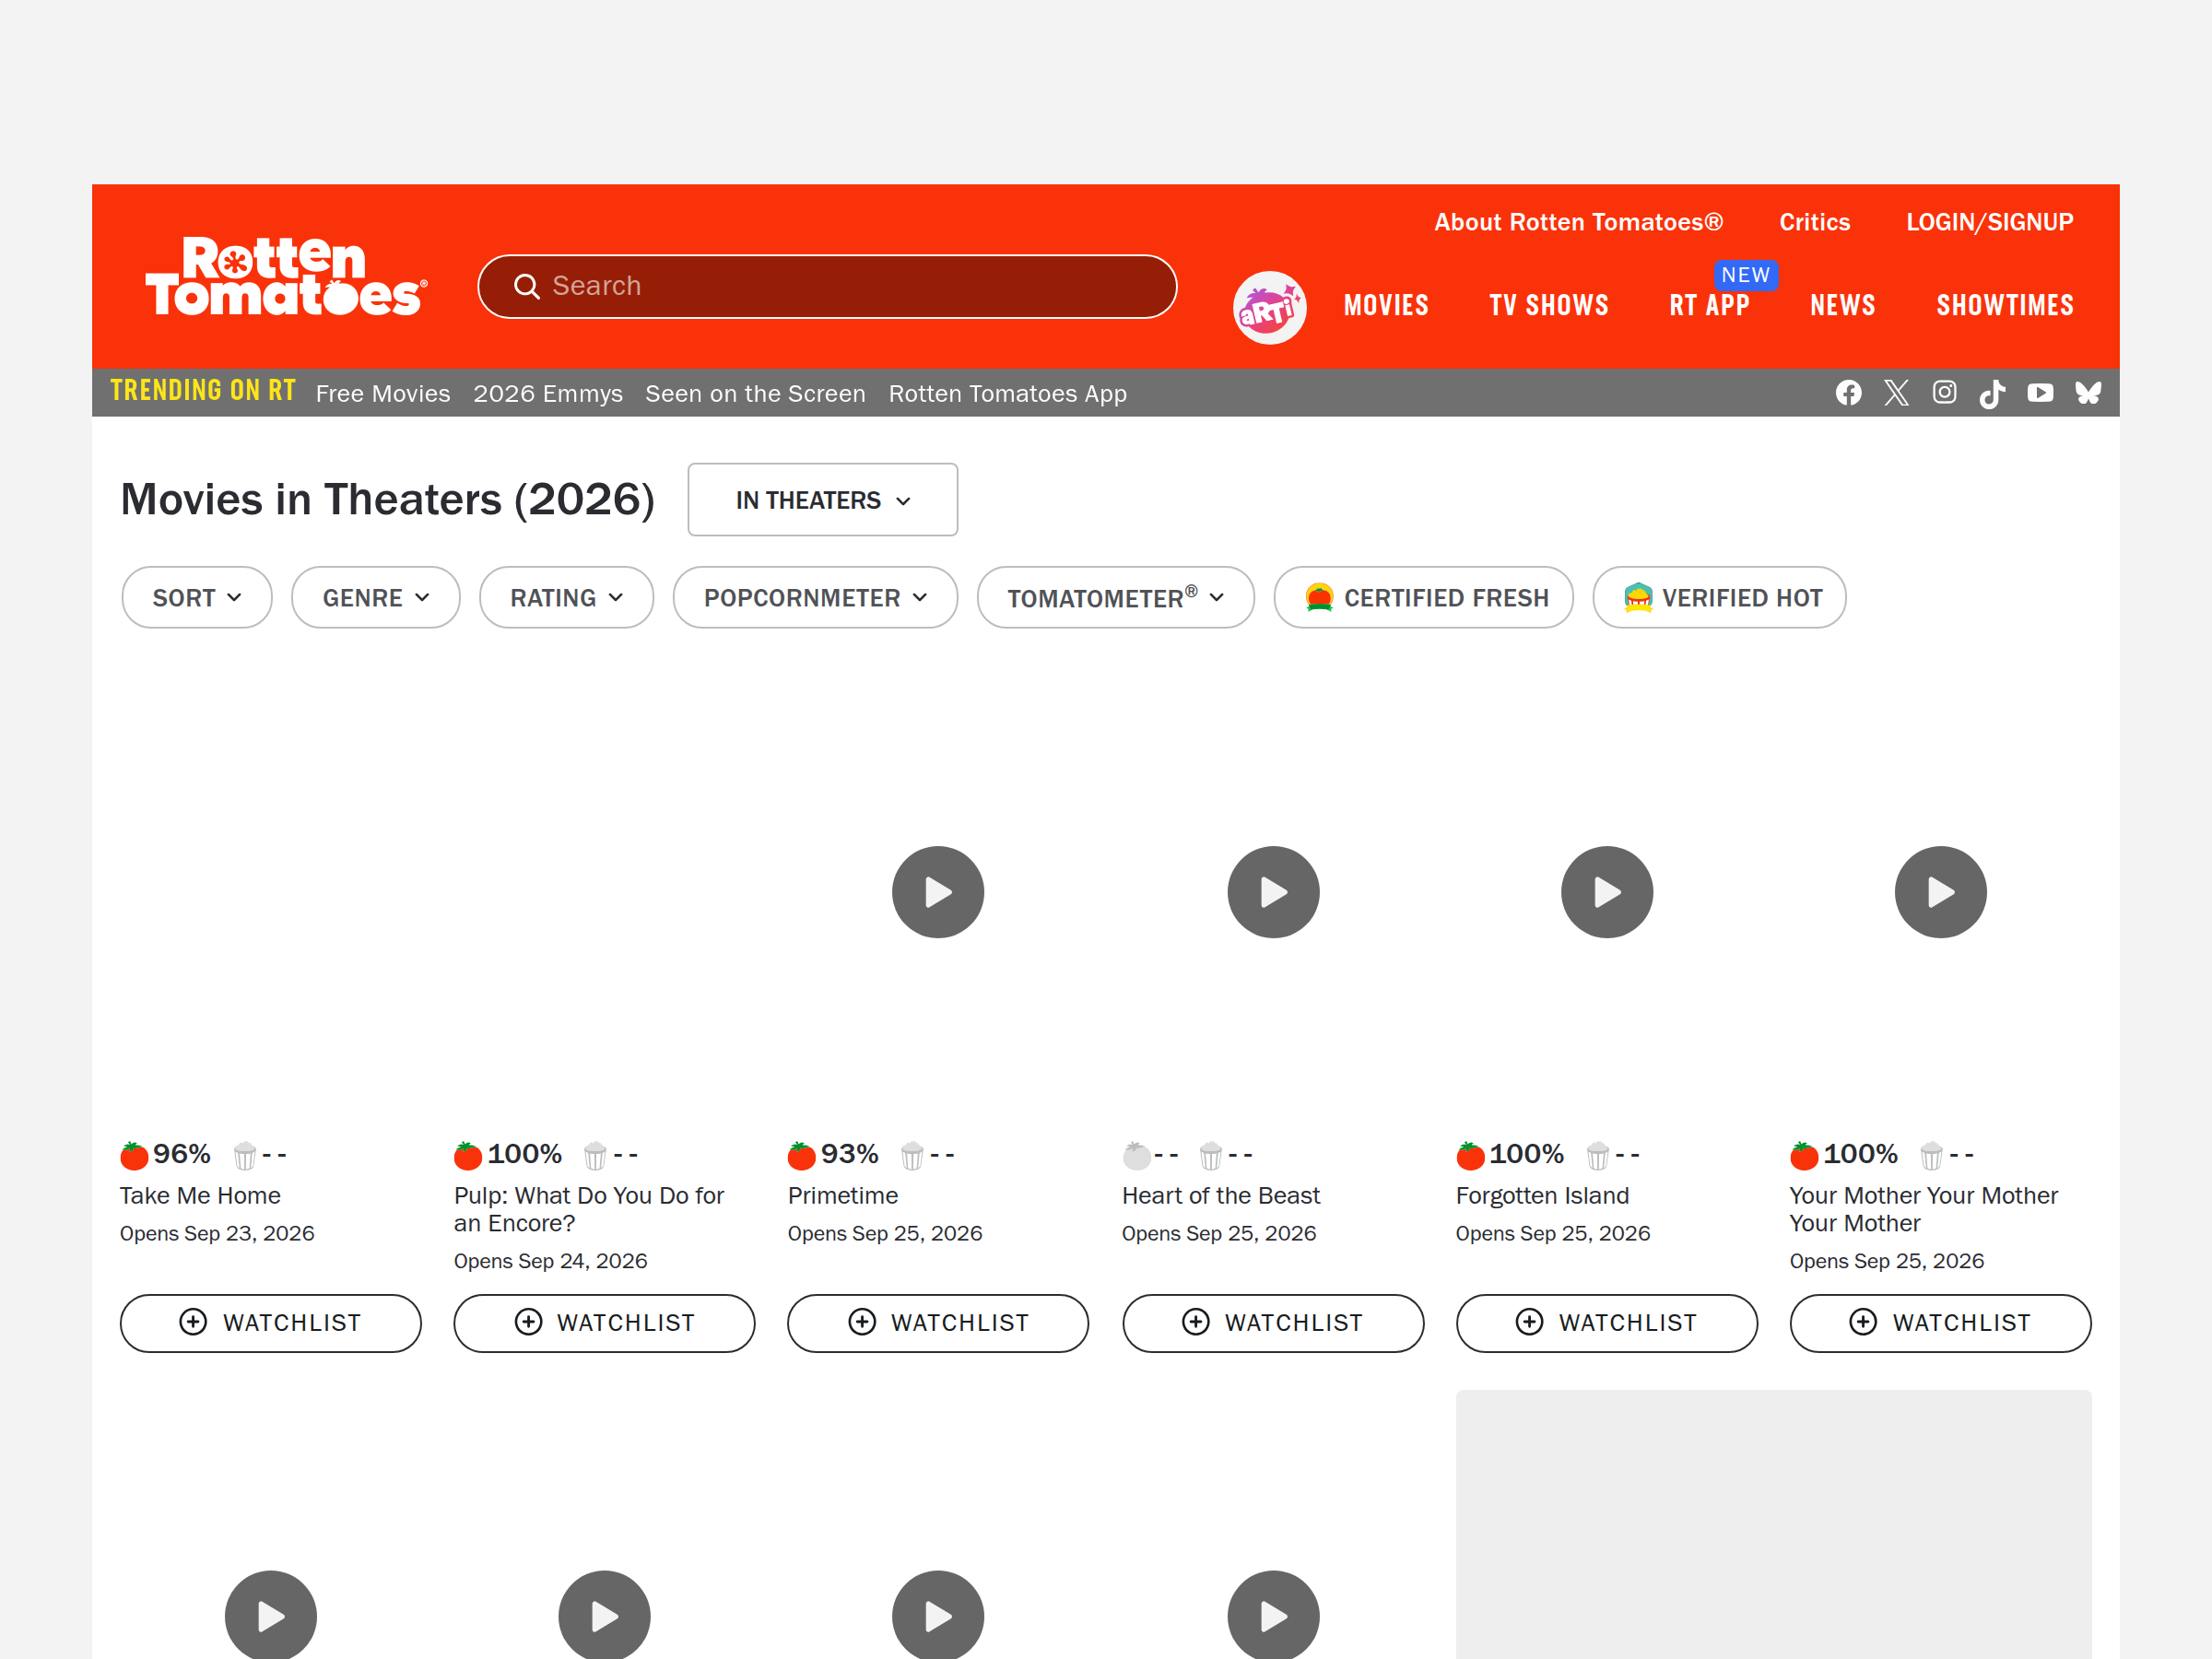
\includegraphics[width=\textwidth]{img/rt_movie_tiles.png}\\
            {\scriptsize rottentomatoes.com --- a differently-shaped card.}
        \end{column}
    \end{columns}
\end{frame}

\begin{frame}{Strategy 8 --- when ``static'' isn't}
    \begin{columns}[T]
        \begin{column}{0.6\textwidth}
            Every strategy so far assumes the HTML you fetch already contains the data you want. IMDb's own film pages break that assumption: a plain \texttt{requests.get()} against an IMDb title page returns HTTP \textbf{202} with \textbf{zero bytes} of body --- not ``missing the cast list,'' completely empty.

            \bigskip

            The real content is built by JavaScript after a browser loads the page, and \texttt{requests} never runs JavaScript. A real browser sees the fully populated page on the right; a script using \texttt{requests} sees nothing at all.

            \bigskip

            We come back to this once we've covered how to make a browser do the fetching for us.
        \end{column}
        \begin{column}{0.35\textwidth}
            \centering
            
\includegraphics[width=\textwidth]{img/imdb_rendered.png}\\
            {\scriptsize What a browser renders. \texttt{requests} gets 0 bytes.}
        \end{column}
    \end{columns}
\end{frame}

\begin{frame}{Which strategy, and where on the spectrum?}
    \begin{columns}[T]
        \begin{column}{0.6\textwidth}
            In pairs, without writing any code: for each site below, name the strategy you'd reach for first, and place it on the 2$\times$2.
            \begin{enumerate}\small
                \item A film festival's ``official selections'' page --- posters and captions, no table
                \item A newspaper's weekly bestseller list, archived and unchanging since 1995
                \item IMDb's ``Top 250'' list page
                \item A directory of every country's population, sourced from three different national statistics sites
            \end{enumerate}
        \end{column}
        \begin{column}{0.35\textwidth}
            \begin{block}{Discussion}
                \footnotesize Which quadrant of the 2$\times$2 is hardest --- and is it hardest because of the \textit{code}, or because of something else (rate limits, permission, trust in what a source reports)?
            \end{block}
        \end{column}
    \end{columns}
\end{frame}

\begin{frame}{In the notebook}
    Wednesday's companion notebook pilots all eight strategies in code, one at a time:
    \begin{itemize}\small
        \item \textbf{Strategies 1--3} --- box-office and Wikipedia tables: clean, decoy-hiding, and needs-cleanup
        \item \textbf{Strategies 4--5} --- the Wikipedia infobox pattern, then porting it across a language edition
        \item \textbf{Strategies 6--7} --- Oscars cards, then Rotten Tomatoes' differently-shaped cards
        \item \textbf{Strategy 8} --- watching \texttt{requests} fail against IMDb, live
    \end{itemize}

    \bigskip

    \begin{alertblock}{Connecting to Ch.~2 (Ethics)}
        Before pointing a loop at any site, check its \texttt{robots.txt} and Terms of Service, and reuse \texttt{responsible\_get()} from the ethics chapter. Politeness is not optional.
    \end{alertblock}
\end{frame}

% =========================================================================
\section{Wednesday · Notebook Lab}
% =========================================================================

\begin{frame}[fragile]{Strategy 1 --- the one-line win}
    One table, one call. When the page cooperates, take the win:
\begin{lstlisting}
import pandas as pd

url = "https://www.boxofficemojo.com/weekend/2018W52/"
tables = pd.read_html(url)
print(f"{len(tables)} table(s) found")   # 1 -- no ambiguity here

weekly = tables[0]
print(weekly.head())
\end{lstlisting}
    No \texttt{requests}, no \texttt{BeautifulSoup} --- \texttt{read\_html()} fetches the page itself. Save this reflex for pages that look like Strategy 1; the next one won't be this easy.
\end{frame}

\begin{frame}[fragile]{Strategy 2 --- finding the real table among decoys}
    Retrieve, then find the right table (pages hide data tables among navigation or mobile-layout tables):
\begin{lstlisting}
import requests
from bs4 import BeautifulSoup

url = "https://www.the-numbers.com/box-office-chart/weekly/2018/12/28"
headers = {"User-Agent": "WebDataScience/1.0 (you@colorado.edu)"}
soup = BeautifulSoup(requests.get(url, headers=headers).text, "html.parser")

tables = soup.find_all("table")
for i, table in enumerate(tables):          # inspect each candidate
    print(i, len(table.find_all("tr")), "rows")
\end{lstlisting}
\end{frame}

\begin{frame}[fragile]{The one-line bug that shifts every column}
    \begin{columns}[T]
        \begin{column}{0.6\textwidth}
        Tempting shortcut:
\begin{lstlisting}
# DON'T: silently drops empty cells
row.text.split("\n")
\end{lstlisting}
        Correct --- walk cell by cell so \textbf{empty cells stay aligned}:
\begin{lstlisting}
cells = row.find_all(["td", "th"])
values = [c.get_text(strip=True)
          for c in cells]
\end{lstlisting}
        \end{column}
        \begin{column}{0.35\textwidth}
            A blank header cell (the ``previous rank'' column) is easy to lose.

            \bigskip

            Split-on-newline drops it. Every later value then shifts one column left, so \textbf{Movie} fills with distributor names.

            \bigskip

            The extra line of code buys correctness.
        \end{column}
    \end{columns}
\end{frame}

\begin{frame}[fragile]{Strategy 3 --- cleaning up after \texttt{read\_html()}}
\begin{lstlisting}
import pandas as pd

url = "https://en.wikipedia.org/wiki/List_of_highest-grossing_films"
df = pd.read_html(url, header=0)[0]     # verified by inspection: index 0
print(df.dtypes)                        # "Worldwide gross" parsed as text
\end{lstlisting}
    Expect to spend as long \textbf{cleaning} as extracting:
\begin{lstlisting}
# a stray footnote-reference letter can sit in front of the "$" --
# print a few raw values first so you know what you're stripping
df["gross"] = pd.to_numeric(
    df["Worldwide gross"].str.replace(r"[^0-9]", "", regex=True), errors="coerce")
df["footnote_count"] = df["Ref"].str.count(r"\[")   # "[# 3][# 4]" -> 2
\end{lstlisting}
\end{frame}

\begin{frame}[fragile]{Strategy 4 --- the infobox pattern}
    A table without a useful class name, but a very reliable shape --- one \texttt{<th>}/\texttt{<td>} pair per row:
\begin{lstlisting}
import requests
from bs4 import BeautifulSoup

url = "https://en.wikipedia.org/wiki/The_Godfather"
headers = {"User-Agent": "WebDataScience/1.0 (you@colorado.edu)"}
soup = BeautifulSoup(requests.get(url, headers=headers).text, "html.parser")

infobox = soup.find("table", class_="infobox")
facts = {}
for row in infobox.find_all("tr"):
    label, value = row.find("th"), row.find("td")
    if label and value:
        facts[label.get_text(strip=True)] = value.get_text(" ", strip=True)
print(facts["Directed by"])   # 'Francis Ford Coppola'
\end{lstlisting}
\end{frame}

\begin{frame}[fragile]{Strategy 5 --- porting the parser to a new site}
    The class name \texttt{infobox} doesn't exist on this page at all. Re-inspect, and anchor on the \texttt{<caption>} instead --- same loop as Strategy 4 after that:
\begin{lstlisting}
url = "https://fr.wikipedia.org/wiki/Le_Parrain_(film)"
soup = BeautifulSoup(requests.get(url, headers=headers).text, "html.parser")

infobox = soup.select("table:has(caption)")[0]   # the anchor that transfers
facts = {}
for row in infobox.find_all("tr"):
    label, value = row.find("th"), row.find("td")
    if label and value:
        facts[label.get_text(strip=True)] = value.get_text(" ", strip=True)
print(facts["Titre original"])   # 'The Godfather' -- same film, new labels
\end{lstlisting}
    The loop is identical. Only the anchor and the labels changed.
\end{frame}

\begin{frame}[fragile]{Strategy 6 --- cards to rows: the Oscars parser}
    Navigate down through the real container hierarchy, category by honoree:
\begin{lstlisting}
area = soup.find("div", class_="field--name-field-award-categories")
categories = area.find_all("div", class_="paragraph--type--award-category")

rows = list()
for cat in categories:
    name = cat.find(class_="field--name-field-award-category-oscars").get_text(strip=True)
    for h in cat.find_all("div", class_="paragraph--type--award-honoree"):
        rows.append({
            "category": name,
            "type": h.find(class_="field--name-field-honoree-type").get_text(strip=True),
            "entity": h.find(class_="field--name-field-award-entities").get_text(strip=True),
        })
df = pd.DataFrame(rows)   # 24 categories on the 2026 ceremony page
\end{lstlisting}
\end{frame}

\begin{frame}[fragile]{Strategy 7 --- a different card, a different site}
    Rotten Tomatoes' tiles are custom elements, not \texttt{<div>}s --- same idea, new anchors:
\begin{lstlisting}
url = "https://www.rottentomatoes.com/browse/movies_in_theaters/"
soup = BeautifulSoup(requests.get(url, headers=headers).text, "html.parser")

tiles = soup.find_all("tile-dynamic", attrs={"data-qa": "tile"})
records = list()
for tile in tiles:
    title = tile.find("span", class_="p--small")
    score = tile.find("rt-text", class_="critics-score")
    records.append({
        "title": title.get_text(strip=True) if title else None,
        "tomatometer": score.get_text(strip=True) if score else None,
    })
# join records on title with the Oscars/box-office DataFrames -- one row per movie
\end{lstlisting}
\end{frame}

\begin{frame}[fragile]{Strategy 8 --- watching \texttt{requests} fail, live}
\begin{lstlisting}
import requests

url = "https://www.imdb.com/title/tt0068646/"
headers = {"User-Agent": "WebDataScience/1.0 (you@colorado.edu)"}
response = requests.get(url, headers=headers)
print(response.status_code, len(response.text))
# 202 0  -- zero bytes. Not a bad selector: there is nothing here to select.
\end{lstlisting}
    \begin{alertblock}{This is not an error in your code}
        \footnotesize A 202 with an empty body means the server accepted the request and handed back a JavaScript shell instead of a page. \texttt{BeautifulSoup} has nothing to parse. This is the boundary this chapter's strategies don't cross --- dynamic pages get their own week.
    \end{alertblock}
\end{frame}

\begin{frame}[fragile]{Make it reusable --- and defensive}
    Abstract the working parser into a function; keep the \texttt{sleep} in the \textit{caller}, not the function:
\begin{lstlisting}
for year in range(2020, 2027):
    df = scrape_oscar_year(year, headers)   # returns empty DataFrame on failure
    all_years.append(df)
    time.sleep(1)                           # politeness lives in the loop
\end{lstlisting}
    Wrap fragile parsing so one bad page doesn't kill the run:
\begin{lstlisting}
try:
    response.raise_for_status()
except requests.RequestException as e:
    print(f"Request failed: {e}"); return None
# AttributeError fires when .find() returns None and you call .text on it
# -- the single most common scraping error.
\end{lstlisting}
    \begin{alertblock}{Error flavors}
        \footnotesize Some code here is \textit{designed} to break (a guard demonstrating the \texttt{AttributeError} above) --- that does not need a GitHub issue. Other code may be \textit{genuinely} broken: confirm it, then search and file an issue.
    \end{alertblock}
\end{frame}

\begin{frame}{Lab: work these, then show-and-tell}
    \begin{columns}[T]
        \begin{column}{0.6\textwidth}
            Work in pairs. Do these exercises from the notebook:
            \begin{enumerate}\small
                \item Get a Wikipedia table with \texttt{read\_html}. Then make a visualization.
                \item Write a parser for a page that has no table. Record your selectors.
                \item Extend the parser to more than one page. Add a delay, error handling, and a function.
                \item Parse a Wikipedia page that is not in English. Report the encoding problems that you correct.
                \item Download each page one time into \texttt{cache/}. Then parse the files offline.
                \item[6.] \textbf{5617}: examine the Terms of Service and the \texttt{robots.txt} file of two sites. Compare them with \textcite{fiesler2020no}
            \end{enumerate}
        \end{column}
        \begin{column}{0.35\textwidth}
            \begin{block}{Submitting}
                \footnotesize Start in class, finish at home, submit what you got working.

                \smallskip

                Graded on good-faith attempt to complete rather than getting everything working.
            \end{block}
            \begin{block}{Show-and-Tell}
                \footnotesize Bring one of these to class: a bug you could not solve, data you find interesting, or a question for a research design.
            \end{block}
        \end{column}
    \end{columns}
\end{frame}

\begin{frame}[standout]
    Sites redesign without warning.\\
    When a parser breaks, that's not a bug in your code ---\\
    it's the web working as designed.\\[1em]
    {\large Re-inspect, re-hypothesize, re-verify.}
\end{frame}

% =========================================================================
\section{Friday · Textbook Revisions}
% =========================================================================

\begin{frame}{Improving Chapter 6 together}
    \begin{columns}[T]
        \begin{column}{0.6\textwidth}
            Today we make the book better. Each of you opens a \textbf{pull request} against \texttt{ch-06-static-pages.qmd} and reviews a classmate's.

            \bigskip

            The workflow (from Week 1):
            \begin{enumerate}\small
                \item Branch / fork the book repo
                \item Edit the chapter; commit with a clear message
                \item Open a PR describing \textit{what} and \textit{why}
                \item Review two peers' PRs: kind, specific, actionable
            \end{enumerate}

            \bigskip

            Review comments still follow Week 3's claim / link / sharpen taxonomy --- claim what you'll fix, link related issues, sharpen ones missing detail.
        \end{column}
        \begin{column}{0.35\textwidth}
            \centering
            
\includegraphics[width=\textwidth]{img/pr_review.png}
        \end{column}
    \end{columns}
\end{frame}

\begin{frame}{A revision menu for Chapter 6}
    High-value targets --- pick one and scope it to a single PR:
    \begin{itemize}
        \item \textbf{Test the code against live sites.} The Numbers, Wikipedia, the Oscars, and Rotten Tomatoes all drift. Run the notebook, report what broke, and fix the selectors (this is the chapter's own ``A Note on Fragility'').
        \item \textbf{Close a gap in ``Common Issues to Debug.''} Add a worked \texttt{\textbackslash xa0} / non-breaking-space example, or a \texttt{colspan}/\texttt{rowspan} case \texttt{read\_html} mishandles.
        \item \textbf{Add a figure.} An annotated Inspector screenshot, or a diagram of the 2$\times$2 research-design spectrum, would help readers place their own project.
        \item \textbf{Strengthen an exercise.} Add expected output, a rubric, or a starter cell so exercises are self-checking.
        \item \textbf{Extend ``Further Reading.''} A data-journalism scrape (ProPublica, The Markup) tied to the ``Public Interest'' callout.
    \end{itemize}
\end{frame}

\begin{frame}{A good revision, and a good review}
    \begin{columns}[T]
        \begin{column}{0.6\textwidth}
            \begin{block}{A strong PR}
                \begin{itemize}\small
                    \item One focused change, clearly titled
                    \item Explains the problem it fixes
                    \item Builds (\texttt{quarto render}) without errors
                    \item Matches the book's voice and notation
                    \item Discloses any AI assistance
                \end{itemize}
            \end{block}
        \end{column}
        \begin{column}{0.35\textwidth}
            \begin{block}{A strong review}
                \begin{itemize}\small
                    \item Runs / reads the change, not just skims
                    \item Names specifics (line, claim, code)
                    \item Separates ``must fix'' from ``nice to have''
                    \item Is generous --- assume good faith
                    \item Ends with a clear verdict
                \end{itemize}
            \end{block}
        \end{column}
    \end{columns}
    \medskip
    \centering\small Next week: \textbf{Archived web pages} --- scraping the past with the Wayback Machine.
\end{frame}

% =========================================================================
\begin{frame}{Key takeaways}
    \begin{enumerate}
        \item Scraping is a pipeline: \textbf{retrieve $\rightarrow$ inspect $\rightarrow$ anchor $\rightarrow$ extract $\rightarrow$ DataFrame}.
        \item Place your project on the single/multi-site $\times$ consistent/inconsistent spectrum before picking a strategy.
        \item Tables, decoys, infoboxes, and cards are different shapes of the same problem --- finding a reliable anchor.
        \item Abstract into functions, rate-limit in the loop, and code defensively.
        \item Pages change: the durable skill is \textbf{inspect, hypothesize, verify} --- not memorized class names.
    \end{enumerate}
    \bigskip
\end{frame}

\end{document}
